\documentclass[12pt]{ucthesis}

\usepackage{etex}
\usepackage[morefloats=125]{morefloats}
\usepackage[hyphens]{url}
\usepackage[breaklinks=true]{hyperref}

\usepackage{graphicx}
\usepackage{tabularx}
\usepackage{amssymb}
\usepackage{amsmath}
\usepackage[letterpaper]{geometry}
\usepackage[overload]{textcase}
\usepackage{color}
\usepackage[nonumberlist,toc]{glossaries}
\usepackage{wrapfig}
\usepackage{longtable}
\usepackage{morefloats}
\usepackage{float}
\usepackage{listings}
\usepackage{makecell}
\usepackage[titletoc]{appendix}
\usepackage{cleveref}
\usepackage[]{algorithm2e}
\usepackage{amsmath}

\usepackage{subfigure}

%\usepackage{caption}
%\usepackage{subcaption}

% Sets line spacing to double
% \linespread{1.6}

\makeindex
\makeglossaries

\bibliographystyle{abbrv}

\setlength{\parindent}{0.25in} \setlength{\parskip}{6pt}
\geometry{verbose,nohead,tmargin=1in,bmargin=1in,lmargin=1.5in,rmargin=1in}
\setcounter{tocdepth}{2}

% Different font in captions (single-spaced, bold) ------------
\newcommand{\captionfonts}{\small\bf\ssp}

\newcommand{\mycaption}[2]{\caption[#1 --- #2]{#1 --- #2}}

\makeatletter  % Allow the use of @ in command names
\long\def\@makecaption#1#2{%
  \vskip\abovecaptionskip
  \sbox\@tempboxa{{\captionfonts #1: #2}}%
  \ifdim \wd\@tempboxa >\hsize
    {\captionfonts #1: #2\par}
  \else
    \hbox to\hsize{\hfil\box\@tempboxa\hfil}%
  \fi
  \vskip\belowcaptionskip}
\makeatother   % Cancel the effect of \makeatletter
% ---------------------------------------

% Define Appendix refs
\crefname{app}{appendix}{appendices}
\Crefname{app}{Appendix}{Appendices}

\widowpenalty10000
\clubpenalty10000

\begin{document}

%COMMENT BELOW TO OUTPUT WORKING DRAFT
%COMMENT BELOW TO OUTPUT WORKING DRAFT
%COMMENT BELOW TO OUTPUT WORKING DRAFT

%% Declarations for Front Matter
%\title{Class F Amplifier}
\author{Tannis Hodge}
\degreemonth{June} \degreeyear{2016} \degree{Master of Science}
\defensemonth{June} \defenseyear{2016}
\numberofmembers{2}
   \chair{Professor Alexander Dekhtyar, Ph.D. \linebreak Department of Computer Science}
   \othermemberA{Associate Professor Aaron Keen, Ph.D. \linebreak Department of Computer Science}
   \othermemberB{Professor Franz Kurfess, Ph.D. \linebreak Department of Computer Science}
\field{Electrical Engineering} \campus{San Luis Obispo}
\copyrightyears{seven}

%
%\maketitle
%
%\begin{frontmatter}
%
%% Custom made for Cal Poly (by Mark Barry, modified by Andrew Tsui).
%\copyrightpage
%
%% Custom made for Cal Poly (by Andrew Tsui).
%\committeemembershippage
%
%\begin{abstract}
%Your abstract goes in here

%\end{abstract}
%
%\begin{acknowledgements}
%\noindent
Thanks to:
\begin{itemize}
    \item Andrew Guenther, for uploading this template
\end{itemize}

%\end{acknowledgements}
%
%\tableofcontents
%
%\listoftables
%
%\listoffigures
%
%\end{frontmatter}

%END COMMENT
%END COMMENT
%END COMMENT

\pagestyle{plain}
\renewcommand{\baselinestretch}{1.66}

%\chapter{Abstract and IEEE Design Competition Rules}
Telecommunications is the basis of our modern world. There is infrastructure from microwave links, fiber-optic links, and satellite links that connect people all over the world together. Each year more and more data is transferred through these networks. The Cellular Telephone Industries Association reported less than 100 MB of average monthly traffic per smartphone in the United States in 2009 and in 2014 this has jumped up to over 1800 MB of average monthly traffic. To transfer more data, higher order modulation schemes must be used like QAM which require linear amplifiers so amplitude and phase is not distorted during amplification. In portable devices were battery life is one of the key parameters, high efficiency power amplifiers are important due to the large power consumption of the RF amplifiers.

 The International Microwave Symposium (IMS) 2016 High Efficiency Power Amplifier Student Design competition focuses on maximizing the power added efficiency (PAE) and operating frequency of the amplifier over a wide range of input powers. Power added efficiency is defined as the difference of output RF power and RF input power over the DC bias power seen in Equation \ref{eq:pae}. PAE is an important metric for power amplifiers to show how efficient the amplifier is converting the DC power into RF power, ideally converting 100\%.

\begin{equation}\label{eq:pae}
  PAE,\% = \frac{RF\;Power_{out} - RF\\Power_{in}}{DC\;Power}
\end{equation}

To qualify for the design competition the amplifier must output at least 36 dBm (4 Watts) with less than 24 dBm input power for a single carrier and less than 22 dBm per tone for two carriers spaced 5 MHz apart. Also the amplifier must have a carrier-to-intermodulation ratio (C/I), defined as the ratio in dB between the amplitude of either carrier and the highest intermodulation product, greater than 30 dB at an input power of 0 dBm.

The rules for the amplifier require the amplifier have a center frequency between 1 GHz and 10 GHz. The RF ports should use SMA female connectors, and the bias connections should use banana plugs with a maximum of two DC supply voltages. The source and load impedance of your amplifier should be matched to 50 $\Omega$. The amplifier can use any technology but must be the result of new design and fabrication methods. The amplifier PAE will be measured with at the first RF output power when the C/I ratio drops below 30 dB. The winning amplifier will have the highest figure of merit seen in Equation \ref{eq:fom}. 

\begin{equation}\label{eq:fom}
  Figure of Merit = PAE*(Center Frequency, GHz)^{0.25}
\end{equation}

A table of past competition winners can be seen in Table \ref{table:past_amp_val}. The highest scores in the competition have all been from class F amplifiers with a center frequency around 3.5 GHz with the best amplifier in the competitions past scoring 109.2 at a center frequency of 3.475 GHz and a PAE of 80.1\% in 2011. Since 2011 the winning figure of merit has dropped by more than 20 points. The author thinks that in 2011 and earlier the amplifiers were scored at their highest PAE. And from 2012 on, the amplifiers were scored at the input power when the C/I ratio drops below 30 dB. The class F amplifier was chosen for the design due to highest PAE compared to other amplifier classes and because the design could be accomplished solo within an academic year. Most of the submissions were a group effort, especially the Doherty amplifiers which use a combination of two discrete amplifiers in the design. As per the rules, the amplifier has to be a result of a new effort and this work explores coupling the stubs of the harmonic matching networks to reduce the electrical size of the amplifier using a gallium nitride (GaN) high electron mobility (HEMT) transistor.

\begin{table}
    \centering

    \label{table:past_amp_val}
    \caption{Table of Past Competition Winners and Amplifier Parameters}

    \begin{tabular}{|l|l|l|l|l|l|}
      \hline
      % after \\: \hline or \cline{col1-col2} \cline{col3-col4} ...
      {Year} & {Device} & {Class} & {Frequency, GHz} & {PAE, \%} & {Figure of Merit} \\ \hline
%      2005 & {GaAs FET} & {N/A}     & {1.5}   & {61.7} & {68.3} \\ \hline
      2006 & {Si LDMOS} & {$F^{-1}$}  & {1}     & {75.9} & {75.9} \\ \hline
      2007 & {GaN HEMT} & F         & {1.21}  & {82.9} & {87.0} \\ \hline
      2008 & {GaN HEMT} & {$F^{-1}$}  & {3.2}   & {71.9} & {96.1} \\ \hline
      2009 & {GaN HEMT} & {$F^{-1}$}  & {3.27}  & {71.1} & {95.6} \\ \hline
      2010 & {GaN HEMT} & {J}       & {3.5}   & {74.7} & {102.1} \\ \hline
      2011 & {GaN HEMT} & F         & {3.475} & {80.1} & {109.2} \\ \hline
      2012 & {GaN HEMT} & {Doherty} & {3.5}   & {59.0} & {80.7} \\ \hline
      2013 & {GaN HEMT} & {Doherty} & {3.5}   & {62.5} & {85.5} \\ \hline
      2014 & {GaN HEMT} & {Doherty} & {5}     & {57.8} & {86.4} \\ \hline
      \hline
    \end{tabular}
\end{table}

%
%\chapter{Amplifier Classes}
The generic power amplifier consists of a transistor with a DC bias and AC coupled to the RF input and output ports. For the sake of simplicity this work will only describe the operation of field effect transistor amplifiers. The major source of power consumption of an amplifier comes from the drain source current and voltage that occurs during operation. Power amplifiers come in a variety of classes, and the most commonly used ones are A, B, AB, C, D, E, and F. Classes A through C can be described by the conduction angle of the device and modeling the transistor as a current source. The conduction angle is the amount of current flowing through the transistor from drain to source during a single cycle of the AC signal being amplified and ranges from 0 to $2\pi$ \cite{Colantonio1998}. Classes D through F are defined as switching amplifiers and vary due to the matching networks which shape the waveforms of the current and voltage at the drain and gate of the device \cite{Sokal1975}. This chapter will describe a high level overview of the various amplifier classes and discuss the limitations of each in practice.

%For class A, the conduction angle is $2\pi$ meaning current is always flowing when the amplifier is on increasing the power consumption. Class A does have the advantage of having the highest gain at a given frequency compared to other classes and also can operate near the frequency limit of a transistor .\cite{} Class A also has the highest linearity, lowest harmonic distortion, and is advantageous when high dynamic range is required .\cite{C.Cripps2006} Class B has a conduction angle of $\pi$ so current only flows during half the cycle of the AC signal reducing power consumption. Class AB has a conduction angle between $\pi$ and $2\pi$. Class E is a type of harmonic termination that uses capacitive terminations at the output to achieve 100\% efficiency.

% Citations are wrong above!

\section{Efficiency of Amplifiers}

To reduce the power consumption of a power amplifiers, two major concepts are important: zero voltage switching (ZVS) and zero voltage derivative switching (ZVDS). ZVS is when there is zero voltage when the amplifier is switched on and conducting so while current flows through the output no power is consumed. ZVDS is when there is no overlap between the voltage and current waveforms so no power is consumed during the switching. An amplifier can be 100\% if it achieves ZVS and ZVDS because no power would be consumed at any point in the amplification process. A measure of amplifier efficiency is the power added efficiency (PAE) defined in Equation \ref{pae}. PAE is a measure of how efficient an amplifier is able to convert the input DC power into RF power gain. Ideally all of the DC power used to power the amplifier would be used to increase the input RF power. The maximum limit for a lossless system is 100\%, for example if a power amplifier consumed 1 Watt and was able to output 1.001 Watt of RF power from 1 mW of RF input power, the PAE would be 100.\% because all of the DC power was used to increase the RF power.

\begin{equation}\label{pae}
  PAE,\% = \frac{RF\;Power_{out} - RF\\Power_{in}}{DC\;Power}
\end{equation}

Another measure of amplifier efficiency is the drain efficiency which is the proportion of the output power of the fundamental harmonic over the DC power consumed seen in Equation \ref{drain_eff}. The drain efficiency is typically used when talking about the theory behind the different amplifier classes. In practice, PAE is used as the metric to compare power amplifier efficiency because it takes in account RF input power which is relatively large compared to small signal amplifiers. Small signal amplifiers operate at a bias point that can be assumed to be linear for small input powers. Power amplifiers are large signal devices that operate in the non-linear regions of transistor.

\begin{equation}\label{drain_eff}
  \eta, \% = \frac{P_{Fundamental}}{DC\;Power}
\end{equation}

\section{Current Source Amplifiers}

\subsection{Class A Amplifier}

\begin{figure}
  \centering
  % Requires \usepackage{graphicx}
  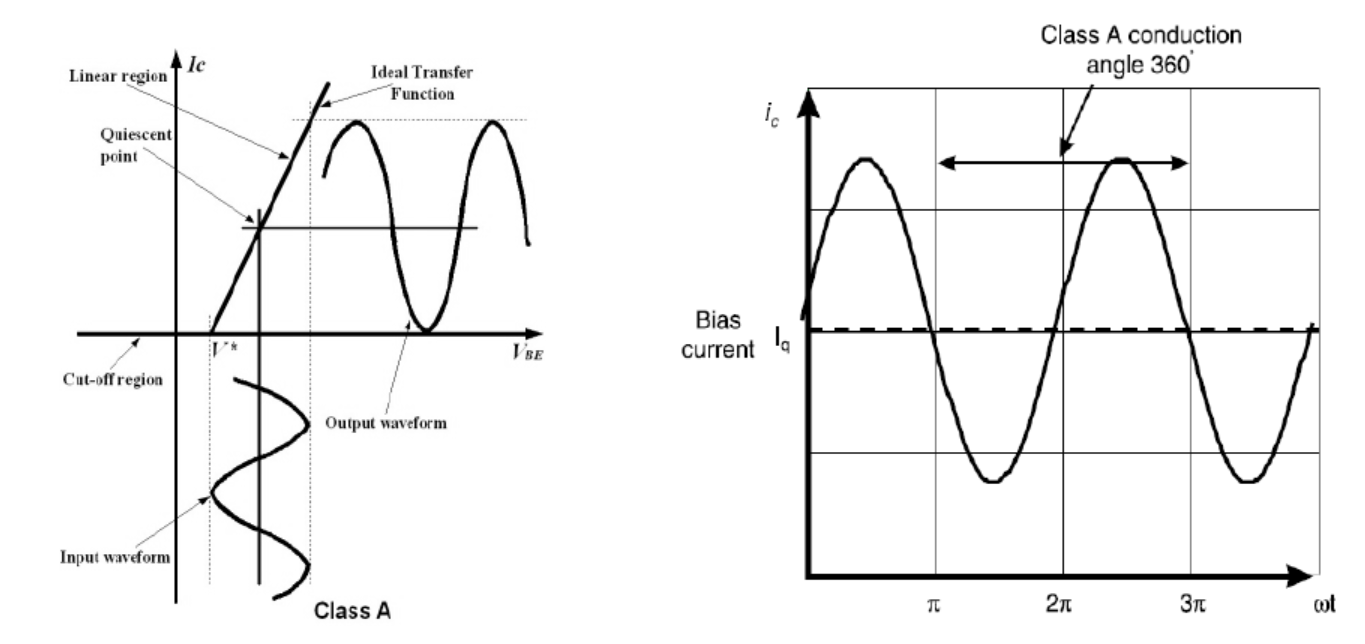
\includegraphics[width=6in]{figures/classes/classa}
  \caption{Class A Bias Point and Conduction Cycle \cite{Rosu2001}}\label{classa_bias}
\end{figure}

The class A amplifier uses a bias that results in a conduction angle of $2\pi$, seen in Figure \ref{classa_bias}, and a theoretical quiescent current of 50\% the maximum drain current. This results in power always being consumed due to the constant bias current and voltage present at the drain of the amplifier. The bias point is chosen so the transistor operates in the active region which can be seen in Figure \ref{classa_bias}. The constant power consumption limits the maximum efficiency of the class A amplifier for a continuous wave (CW) signal to 50\% \cite{C.Cripps2006}.

%The class A amplifier is similar to the small signal amplifier in many ways

The class A amplifier is the most linear of all classes due to the conduction angle that provides ideally no clipping of the current or voltage waveforms. The high linearity allows the class A amplifier to have the lowest intermodulation distortion (IMD) of all the amplifier classes. The downside of the linearity is that the input drive level is proportional to the IMD present at the output of the amplifier. Class A amplifiers are also able to operate closer to the highest operating frequency of a transistor because it does't use the harmonics present in the amplifier for it's amplification \cite{Rosu2001}. %ham paper

%Fix all the citations lol


\subsection{Class B Amplifier}

\begin{figure}
  \centering
  % Requires \usepackage{graphicx}
  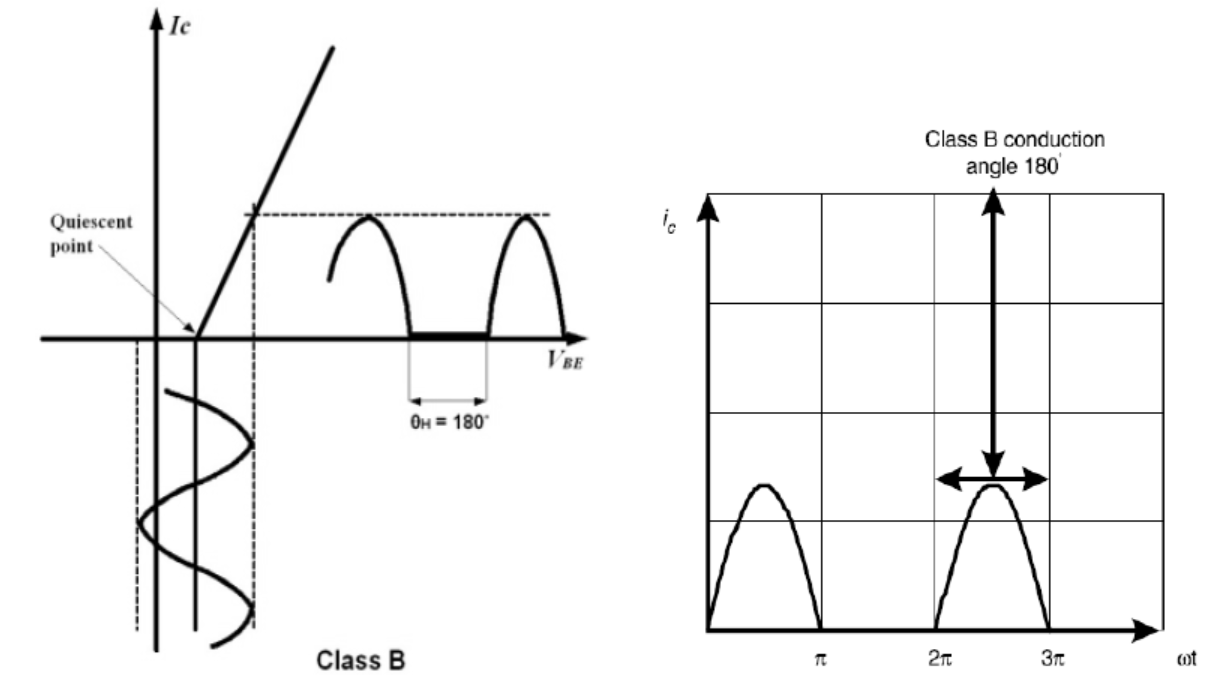
\includegraphics[width=6in]{figures/classes/classb_bias}\\
  \caption{Class B Bias Point and Conduction Cycle \cite{Rosu2001}}\label{classb_bias}
\end{figure}

Class B uses a conduction angle of $\pi$ resulting in a half sinusoid waveform for the drain current seen in Figure \ref{classb_bias} with a theoretical quiescent current of 0 A. The maximum efficiency for a CW signal is 78.5\%. The reduced conduction angle causes the required input power to achieve the maximum efficiency to be 6 dB higher compared to the class A amplifier \cite{C.Cripps2006}.
The drain current is proportional to the input signal so the Class B amplifier is considered a linear amplifier but will result in harmonic distortion due to the clipping of the drain current. The output is usually filtered to reduce the harmonic distortion\cite{Raab2003}.
In most applications, the class B amplifier is used in a push pull configuration to reduce distortion by providing a full sine wave output and maintain greater efficiency than a class A amplifier. Also instead of setting the quiescent current to 0, the drain current is typically set to 10\% of the max drain current of the transistor to reduce the harmonic distortion. An interesting result of the push pull configuration is that even harmonics subtract one another out while odd harmonics add together \cite{Rosu2001}.


\subsection{Class AB Amplifier}

\begin{figure}
  \centering
  % Requires \usepackage{graphicx}
  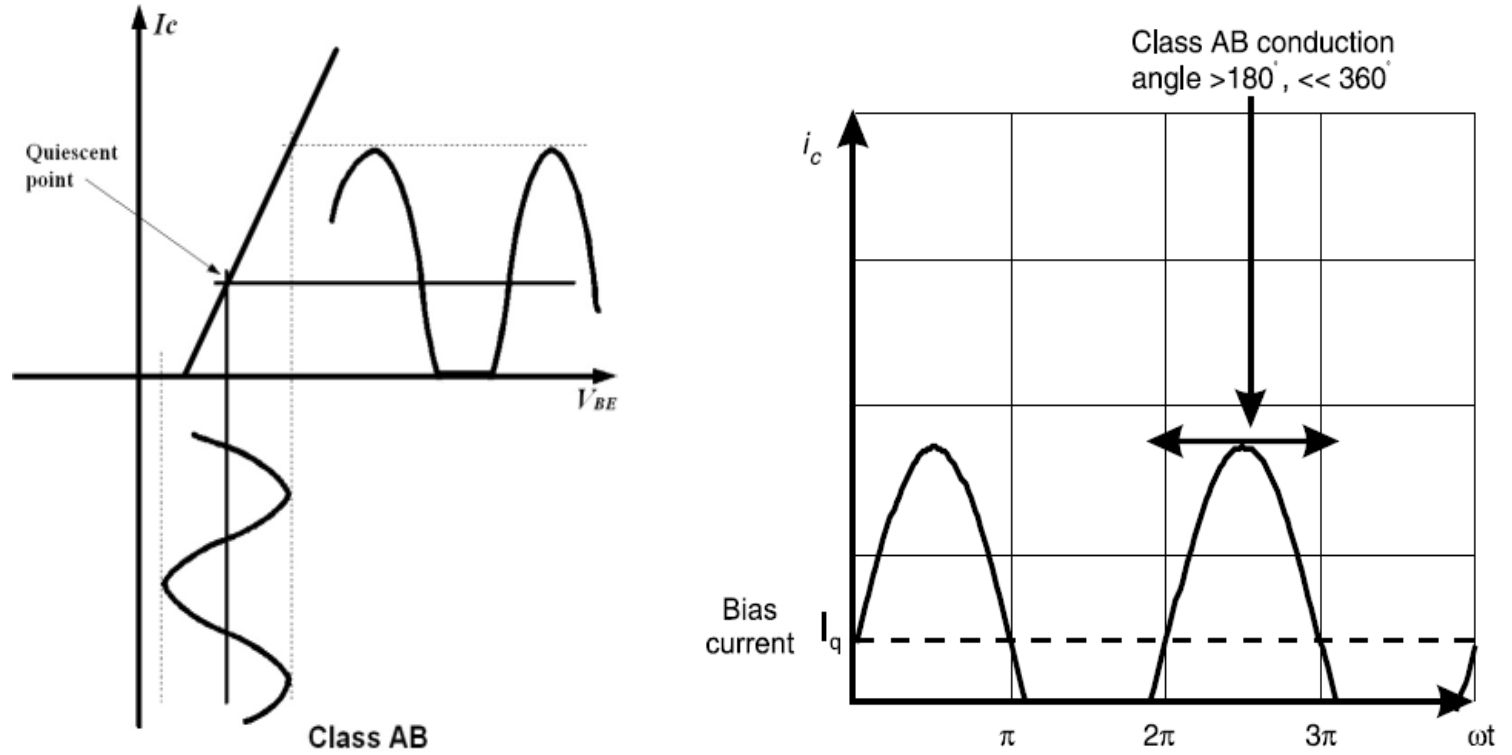
\includegraphics[width=6in]{figures/classes/classab_bias}\\
  \caption{Class AB Bias Point and Conduction Cycle \cite{Rosu2001}}\label{classab_bias}
\end{figure}

The class AB amplifier uses a conduction angle ranging between $\pi$ and $2\pi$ and is a compromise between class A and class B amplifiers. The drain efficiency lies between 50\% and 78.5\% with approximately the same output power as the class A amplifier \cite{C.Cripps2006}. The bias point and conduction cycle can be seen in Figure \ref{classab_bias}. The class AB amplifier offers a wider dynamic range than class A or class B because the conduction angle is proportional to the drain current which also results in the class AB amplifier being a non-linear amplifier \cite{C.Cripps2006}.

\subsection{Class C Amplifier}

\begin{figure}
  \centering
  % Requires \usepackage{graphicx}
  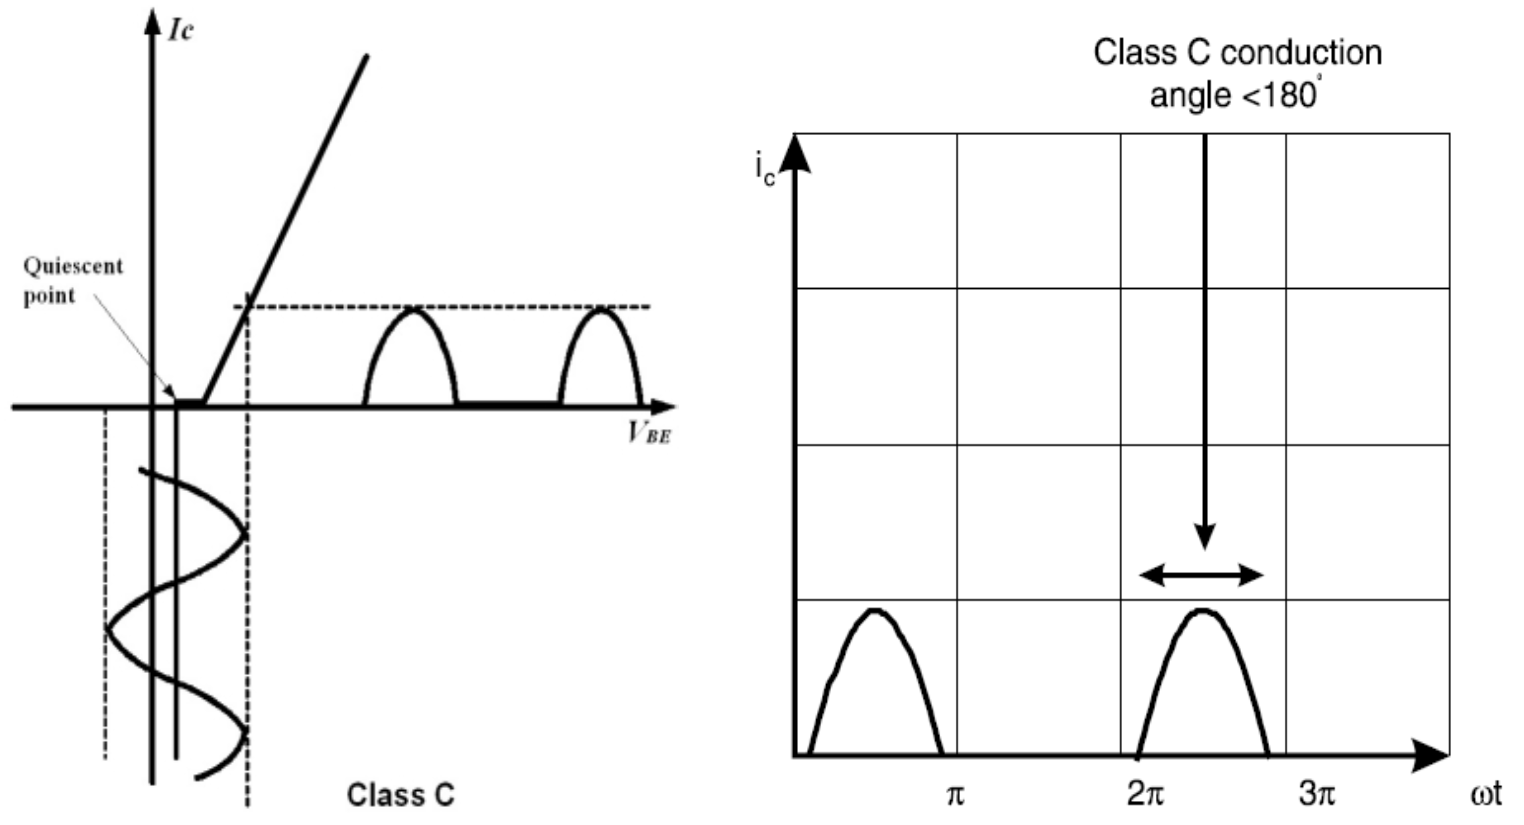
\includegraphics[width=6in]{figures/classes/classc_bias}\\
  \caption{Class C Bias Point and Conduction Cycle \cite{Rosu2001}}\label{classc_bias}
\end{figure}

The class C amplifiers is biased such that the quiescent current is 0 A and the conduction angle is between $0$ and $\pi$ seen in Figure \ref{classc_bias}. The class C amplifier is non-linear with a higher efficiency than class B with a maximum drain efficiency of 100\% at zero conduction angle but will have zero gain. In practice, the class C amplifier has a conduction angle slightly less than $\pi$ for a maximum efficiency of 85\% while still having a useful gain \cite{Raab2003}. The class C has the highest harmonic distortion of all the current source amplifier classes which will be shown in the following section. The harmonic distortion requires significant filtering at the output of the amplifier. Class C amplifiers aren't typically used for microwave power amplifiers due to the large negative voltage present at the gate of the transistor which can cause reverse breakdown in the transistor \cite{C.Cripps2006}. The class C amplifier offers a tradeoff of higher efficiency but with higher harmonic distortion and lower output power level compared to the other current source amplifier classes.

\subsection{Harmonic Distortion}

The current source power amplifiers can be generalized to a power amplifier with various conduction angles and the drain efficiencies. The  output power and harmonic distortion can be described as a function of conduction angle seen in Equations \ref{eq:cond_eff}, \ref{eq:cond_pout}, and \ref{eq:cond_current} \cite{Hella}. Table \ref{table:waveform_param} defines the various parameters to the various equations. Figure \ref{fig:bias_current_harmonic} shows the normalized output current harmonics versus conduction angle. At a conduction angle of $2\pi$, the output has minimal harmonic distortion with only the fundamental and DC component  present. The DC component is easily removed by coupling capacitor. As conduction angle increase, the other harmonic amplitudes increase which causes increased harmonic distortion and the DC power is reduced increasing the efficiency. At zero conduction angle, the transistor won't conduct any current and all of the harmonic amplitudes drop to 0. Figure \ref{fig:bias_power_eff} shows the RF power relative to class A and efficiency versus conduction angle assuming the harmonics are removed and the transistor is optimally loaded. A power amplifier is said to be properly loaded if the load resistance is equal to the DC drain voltage minus the knee voltage of the transistor divided by the fundamental drain current, see Equation \ref{eq:opt_load} \cite{Hella}.

The generalized form of the current source amplifiers are not able to ever achieve ZVS due to the constant drain voltage waveform present at the output which is required to bias the amplifier. And current source amplifiers can only achieve ZVDS at a conduction angle of 0 radians which results in 0 power delivered to the load. To achieve 100\% efficiency and have a practical gain we look to the switching amplifier.
%In the equations, $v_{dd}$ is the drain voltage, $v_{sat}$ is the saturation voltage of the transistor, $\theta$ is the conduction angle in radians,

\begin{table}
    \caption{Table of Current Source Waveform Parameters}
    \label{table:waveform_param}
        \begin{center}
            \begin{tabular}{|l|l|l|}
              \hline
              % after \\: \hline or \cline{col1-col2} \cline{col3-col4} ...
              Parameter & Definition & Units\\ \hline
              $I_m$ & Maximum drain current of transistor & A \\ \hline
              $I_n$ & Magnitude of current harmonic $n$ & A \\ \hline
              $v_{dd}$ & DC drain voltage & V\\ \hline
              $v_{knee}$ & Knee voltage of transistor & V\\ \hline
              $v_{sat}$ & Saturation voltage of transistor & V \\ \hline
              $\theta$ & Conduction angle & Radians\\ \hline

            \end{tabular}
        \end{center}
\end{table}

\begin{equation}\label{eq:cond_eff}
  \eta_{Drain}, \% = \frac{v_{dd} - v_{sat}}{v_{dd}} \frac{\theta - sin\theta}{4(sin\frac{\theta}{2} - \frac{\theta}{2} cos\frac{\theta}{2}) }
\end{equation}

\begin{equation}\label{eq:cond_pout}
  P_{out} = \frac{1}{2}(v_{dd} - v_{sat} )\frac{I_m}{2\pi}(\theta - sin\theta)
\end{equation}

\begin{equation}\label{eq:cond_current}
  I_n = \frac{1}{\pi}\int_{-\frac{\theta}{2}}^{\frac{\theta}{2}} \frac{I_m}{1 - cos(\frac{\theta}{2})} (cos\alpha - cos(\frac{\theta}{2}))cos(n\alpha) \; d\alpha
\end{equation}

\begin{equation}\label{eq:opt_load}
  R_{opt} = \frac{v_{dd}-v_{knee}}{I_{Fundemetnal}}
\end{equation}

\begin{figure}
  \centering
  % Requires \usepackage{graphicx}
  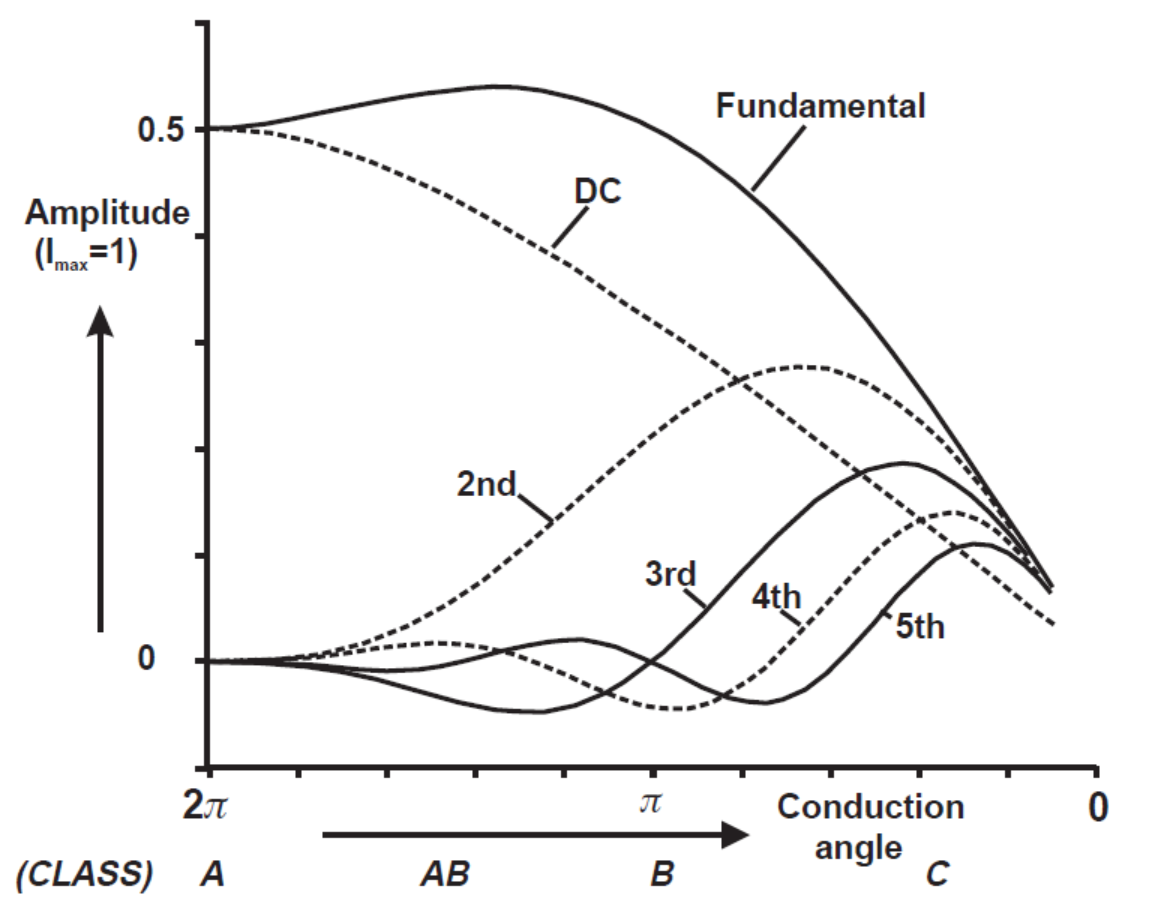
\includegraphics[width=4in,height=4in,keepaspectratio]{figures/classes/bias_current_harmonic}\\
  \caption{Normalized Current Harmonic Amplitude versus Conduction Angle \cite{C.Cripps2006}}
  \label{fig:bias_current_harmonic}
\end{figure}

\begin{figure}
  \centering
  % Requires \usepackage{graphicx}
  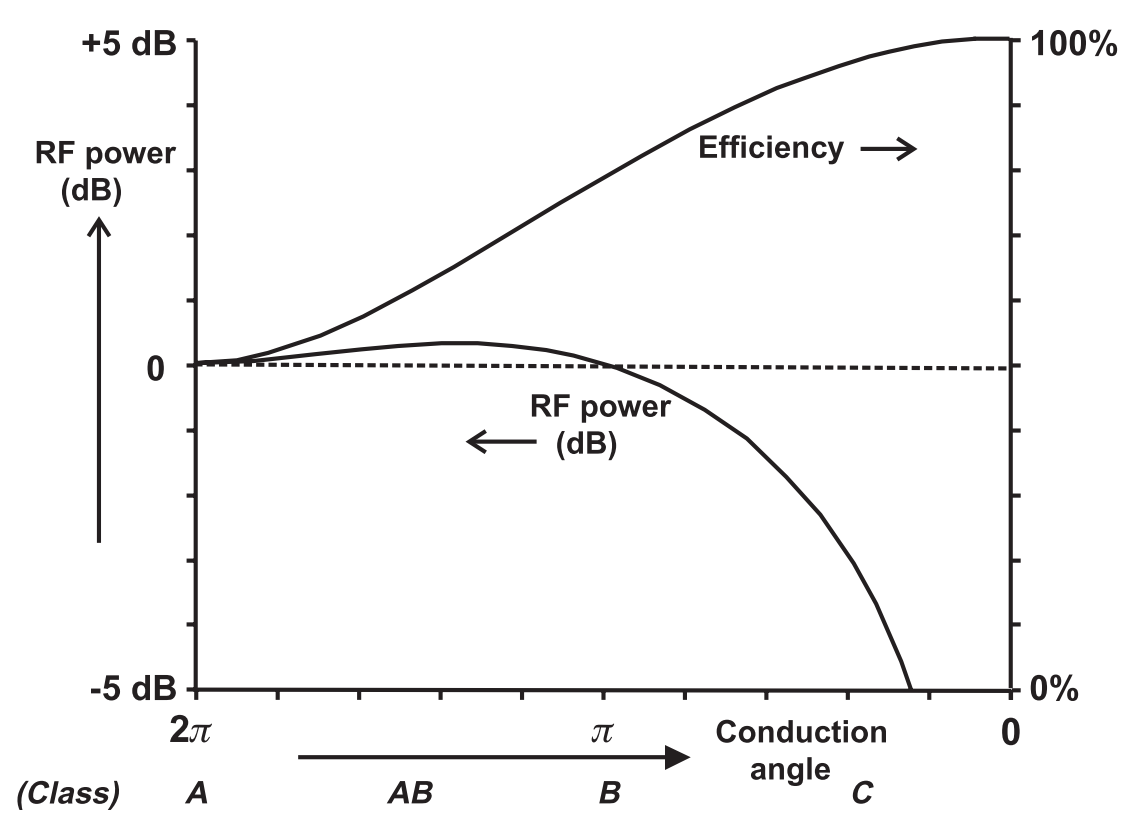
\includegraphics[width=4in,height=4in,keepaspectratio]{figures/classes/bias_power_eff}\\
  \caption{RF Power (relative to Class A) and Efficiency versus Conduction Angle \cite{C.Cripps2006}}
  \label{fig:bias_power_eff}
\end{figure}

\section{Switching Amplifiers}

Switching amplifiers model the transistor as a switch instead a dependent current source. Figure \ref{fig:basic_switch} shows the ideal operation of a switching amplifier. The transistor is modeled as a switch that can only be "on" or "off" depending on the gate voltage. The switching operation allows for current to flow while the switch is on with 0 drain voltage, and for 0 current while the switch is off with a non-zero drain voltage. Ideally this would allow for ZVS and for ZVDS which could result in 100\% efficiency. The switching amplifier classes (D, E, and F) build upon this ideal model and are able to achieve higher efficiencies in practice than current source amplifiers by using matching networks to shape the waveforms at the drain and gate.

\begin{figure}
    \subfigure{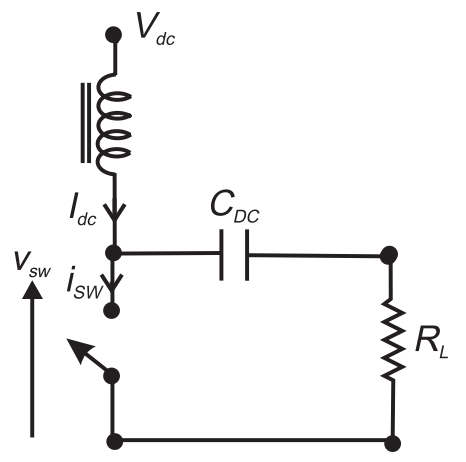
\includegraphics[width=3in]{figures/classes/basic_switch}}
    \subfigure{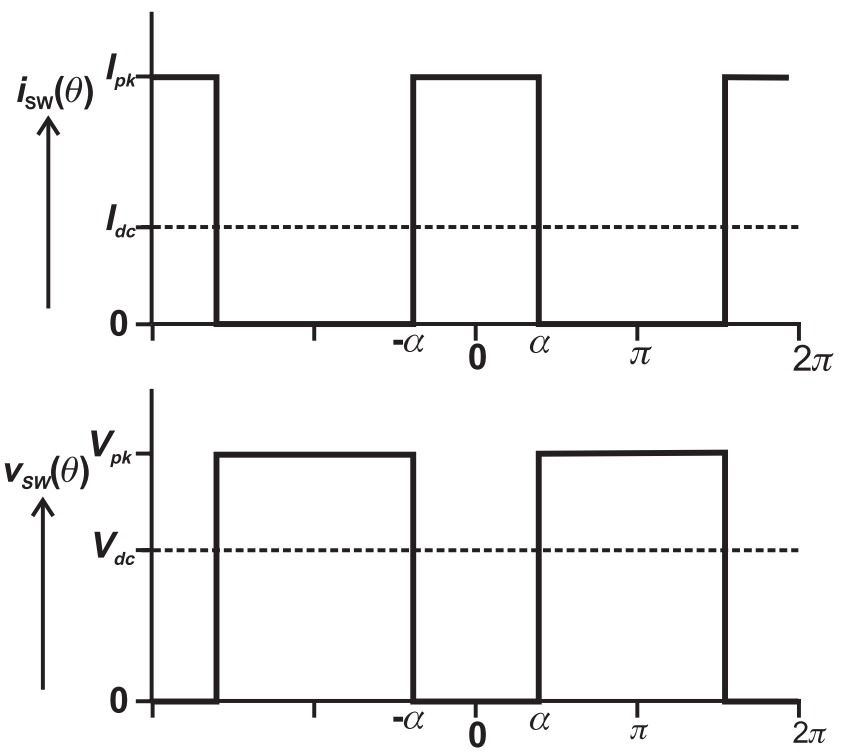
\includegraphics[width=3in]{figures/classes/basic_switch_waveform}}
    \caption{Basic Switching Amplifier Circuit and Waveforms\cite{C.Cripps2006}}\label{fig:basic_switch}
\end{figure}

\subsection{Class D Amplifier}

The class D amplifier can be thought of as push pull version of a switching amplifier. The amplifier consists of two transistors to operate as switches to conduct during the positive half and negative half cycle of the input seen in Figure \ref{fig:class_d} \cite{C.Cripps2006}. This allows for a full wave drain current to flow through the output load that is filtered through a high Q LC network while the drain voltage is a square wave with 0 overlap between the transistor that is on that allows for ZVS and ZVDS \cite{Rosu2001}. This allows the class D amplifier to theoretically have 100\% drain efficiency. The LC network is tuned to the fundamental frequency of the input. Class D looks effective in theory but suffers due to switching resistances and drain capacitances which limit the maximum frequency of operation to VHF in practice \cite{Raab2003}.

\begin{figure}
    \subfigure{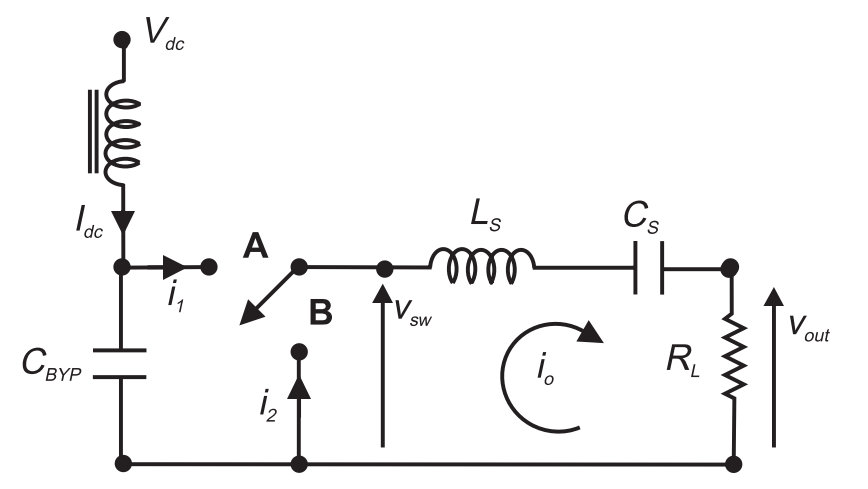
\includegraphics[width=3in]{figures/classes/classd_ckt}}
    \subfigure{{\raisebox{-0.25\height}{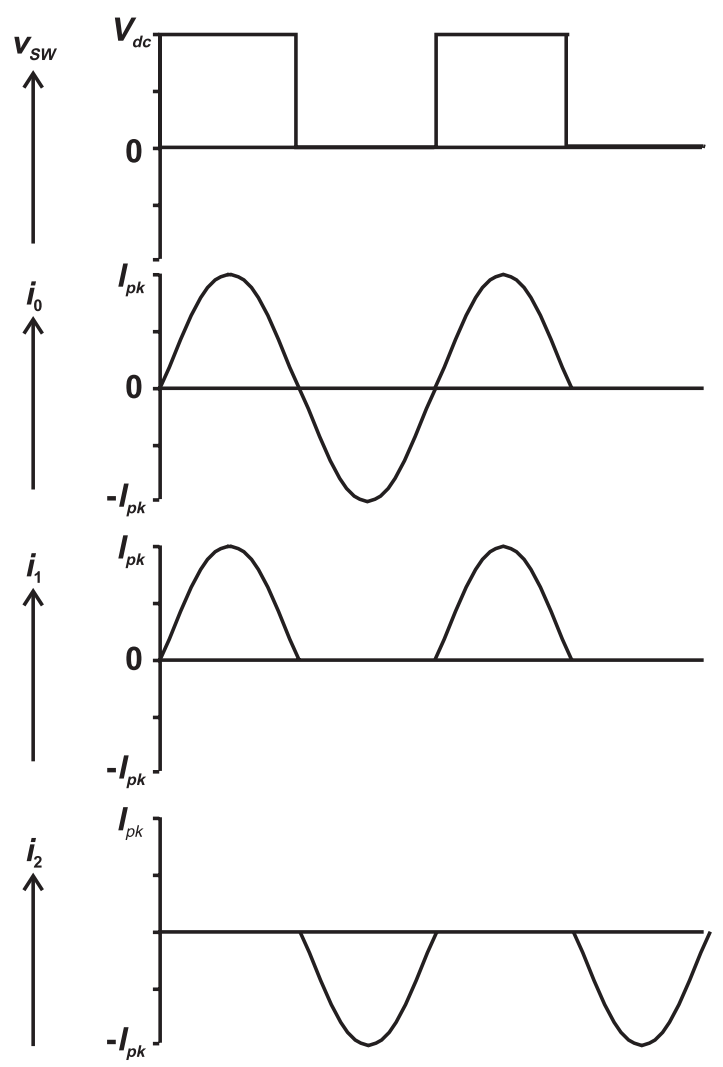
\includegraphics[width=3in,height=3in,keepaspectratio]{figures/classes/classd_wave}}}}
    \caption{Class D Amplifier Circuit and Waveforms\cite{C.Cripps2006}}\label{fig:class_d}
\end{figure}


\subsection{Class E Amplifier}

The class E amplifier builds up on the ideal switch amplifier takes in account for the shunt output drain capacitance and amplification is the result of DC and RF currents that charge the drain shunt capacitance \cite{Raab2003}. As seen in Figure \ref{fig:class_e}, the switch is turned on from  time $-\alpha_1$ to $\alpha_2$ allowing current to flow solely from the power supply and the load through the switch and the voltage across the drain capacitance is shorted. Then as the switch is turned off from time $\alpha_2$ to $\alpha_1$ the current from the power supply and load will flow through the drain capacitor \cite{C.Cripps2006}. To achieve high efficiency, the switching current waveforms are adjusted so that the capacitor current and charge is 0 when the switch is turned on which allows for ZVS and ZVDS conditions allowing for theoretically 100\% efficiency. \cite{Kee2003}.

The class E amplifier produces significant harmonic distortion due to the switching action and the output must be filtered to suppress harmonics \cite{Sokal1975}. Another concern with using the class E amplifier in practice is the large peak voltages at the drain of the transistor which are around three times the drain supply voltage when the switch turns off \cite{Hella}. In addition the output drain capacitance limits the frequency of operation that is required to create the proper drain waveforms \cite{Rosu2001}.

\begin{figure}
    \subfigure{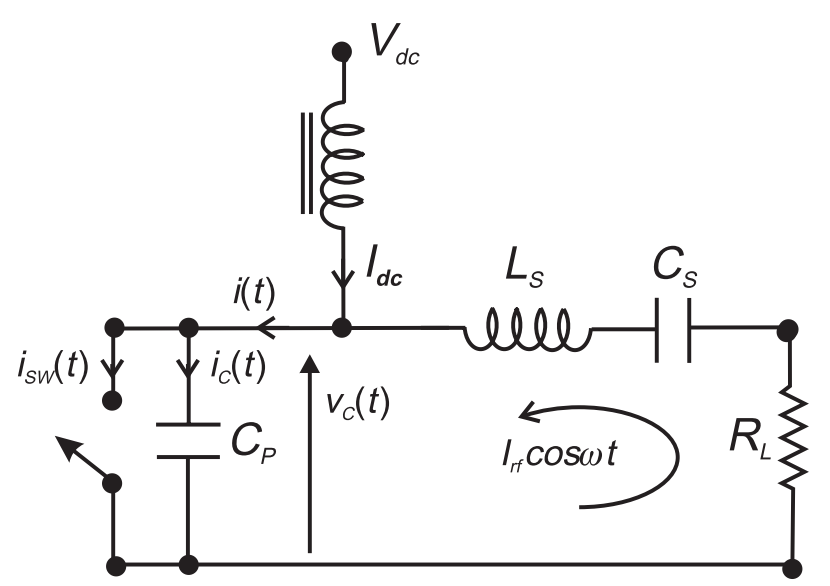
\includegraphics[width=3in]{figures/classes/classe_ckt}}
    \subfigure{{\raisebox{-0.25\height}{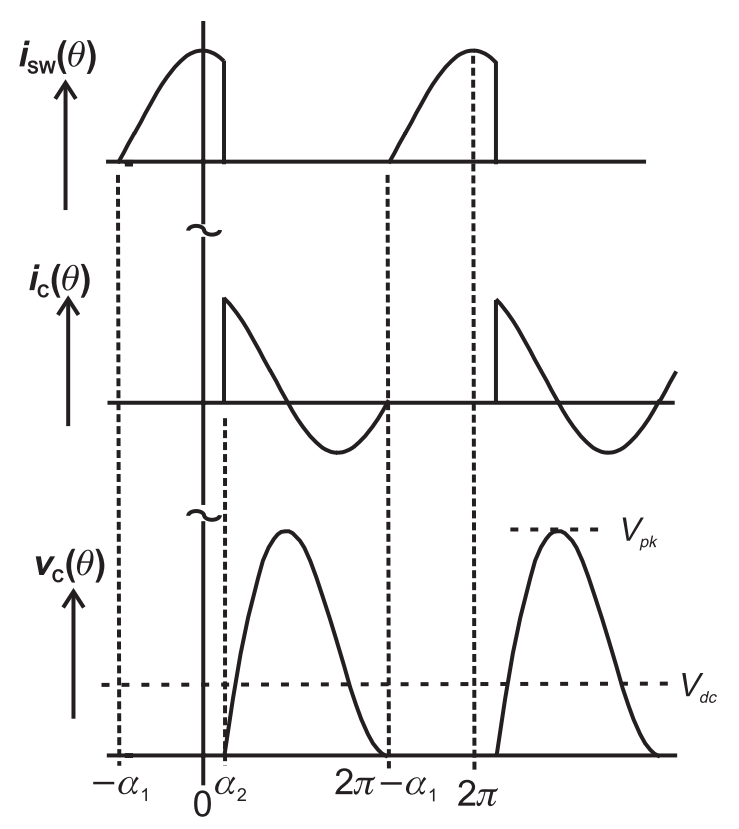
\includegraphics[width=3in,height=3in,keepaspectratio]{figures/classes/classe_wave2}}}}
    \caption{Class E Amplifier Circuit and Waveforms\cite{C.Cripps2006}}\label{fig:class_e}
\end{figure}

\subsection{Class F Amplifier}

The class F amplifier has a theoretical efficiency of 100\% through the use of multi harmonic terminations. The theory behind the class F amplifier relies on the generation of odd voltage harmonics and shorting of even voltage harmonics at the drain of the device to increase the efficiency of the amplifier. By keeping only the odd voltage harmonics of the signal at the output, ideally a square wave would appear and by biasing the amplifier at a conduction angle of pi the amplifier has zero overlap between the current and voltage waveforms and no power consumed when the amplifier is switched on.
The harmonics are generated due to the knee voltage of the transistor. When the AC signal causes the transistor to reach saturation the abrupt change in current flow generates voltage harmonics. In practice it becomes challenging to design matching networks as the number of harmonics to control increases. Also the output capacitance of the transistor will eventually short out higher order harmonics so 100\% efficiency is not realizable in practice. By controlling up to the 5th harmonic, 90.5\% efficiency can be achieved. A more in depth analysis of the class F amplifier follows in the next chapter.

%\subsection{Class J Amplifier}
%
%Shorts even harmonics
%
%Is described by the ratio of the drain reactance and the
%
%Maximum efficiency of 78.5\%


%
%\section{Class F Detailed Description }

\section{Class F Amplifier ADS Simulations, Comparisons to Specs}
%
%\chapter{Class F Amplifier Fabrication and Test Results, Comparisons to Specs}

The final version of the amplifier was milled using the LPFK S62 in the Cal Poly anechoic chamber. One aspect that wasn't taken into account in the ADS simulation was cooling the amplifier during operation. Even when the amplifier is operating at high PAE, it must still dissipate a heat equal to the power that wasn't used to amplify the input signal. The heat dissipation calculations were done assuming the cooling would have to dissipate all of the DC bias power at the highest input power which for the final amplifier was equal to the 170 mA times the bias voltage of 40 V which is equal to 6.8 Watts. The cooling was done with a fan and heatsink mounted on top of the transistor by using the thermal resistance supplied by the manufacturer of the transistor to determine the cooling required. The fan draws 30 mA at 40 volts and was tied to the drain voltage of the amplifier and was included in the PAE measurements of the amplifier. Also to increase the thermal conduction in the final amplifier vias were added underneath the transistor to improve the heat conduction after the board layout was done in ADS. A photo of a previous version of the amplifier that did not have vias can be seen in Figure \ref{fig:old_amp}. Holes were drilled adjacent to the amplifier and copper tape was soldered from the ground pin on the top layer to the bottom layer was used to conduct the heat. The vias proved far superior in conducting heat because they were able to place directly underneath the transistor allowing the heat to be conducted to the ground plane with less thermal resistance.

\begin{figure}
  \centering
  % Requires \usepackage{graphicx}
  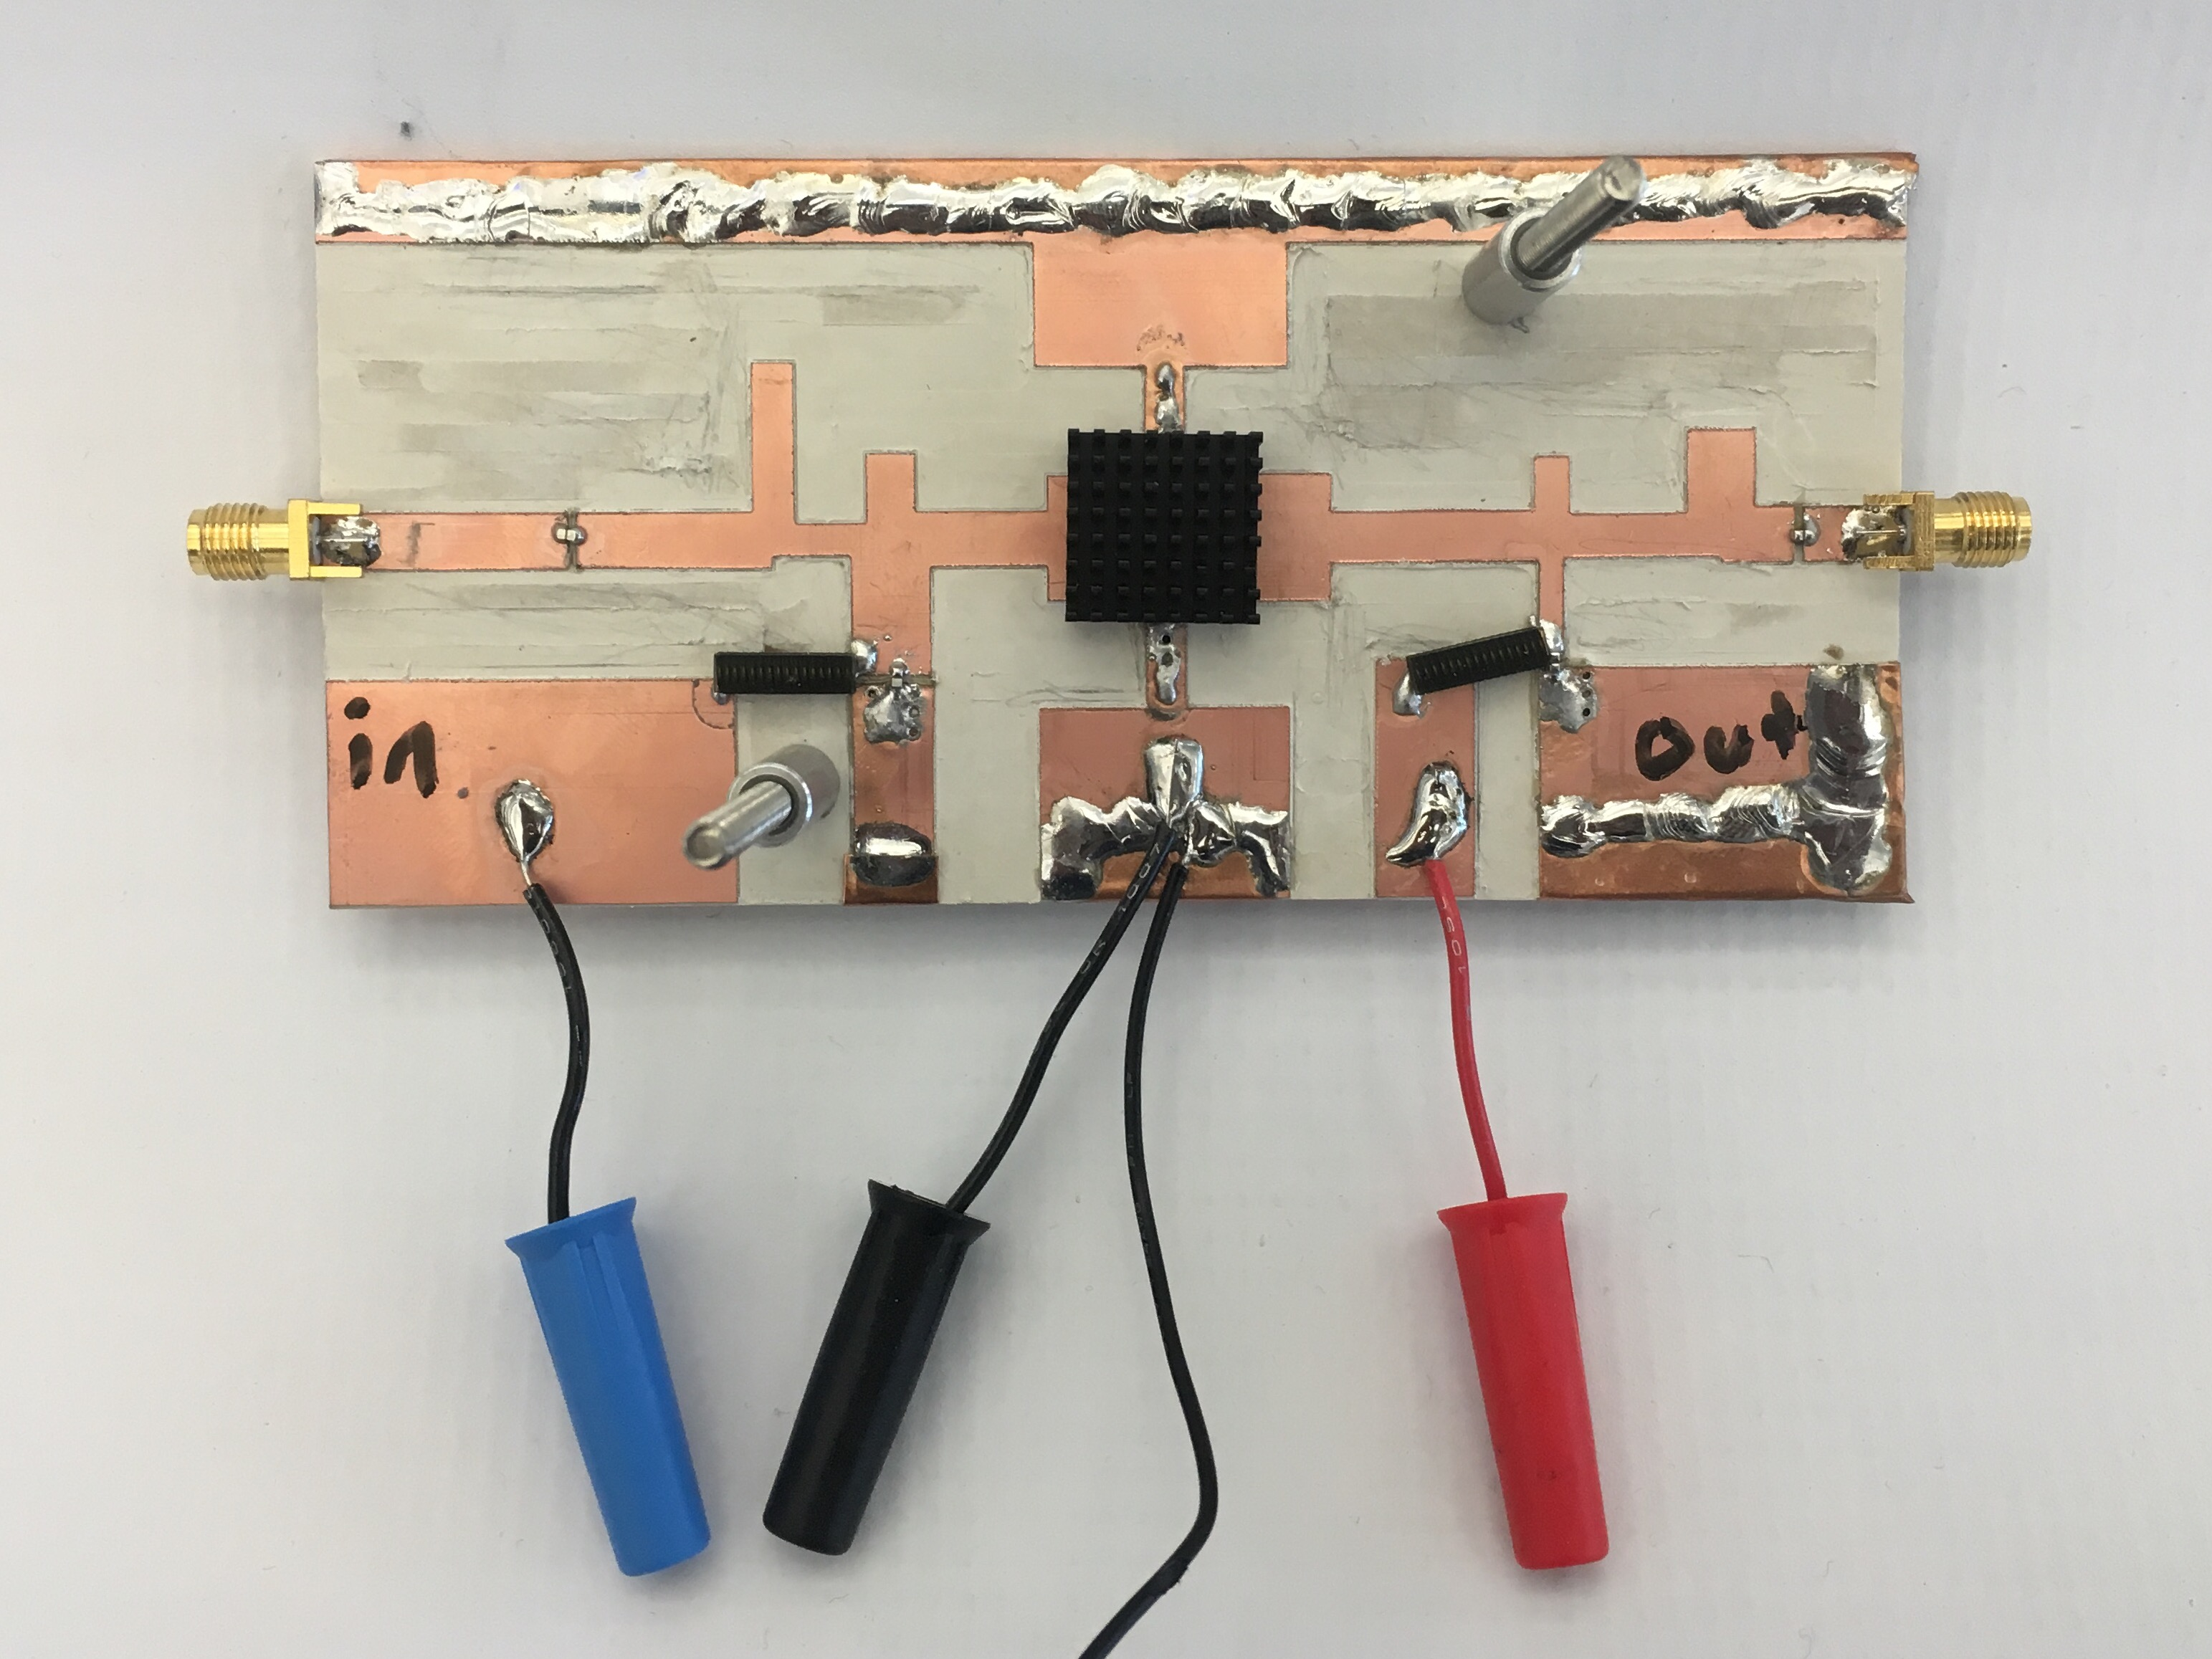
\includegraphics[width=5in,height=5in,keepaspectratio]{figures/test/final_amp}\\
  \caption{Photo of Final Amplifier Without the Fan}
  \label{fig:final_amp}

  \vspace*{\floatsep}

  \centering
  % Requires \usepackage{graphicx}
  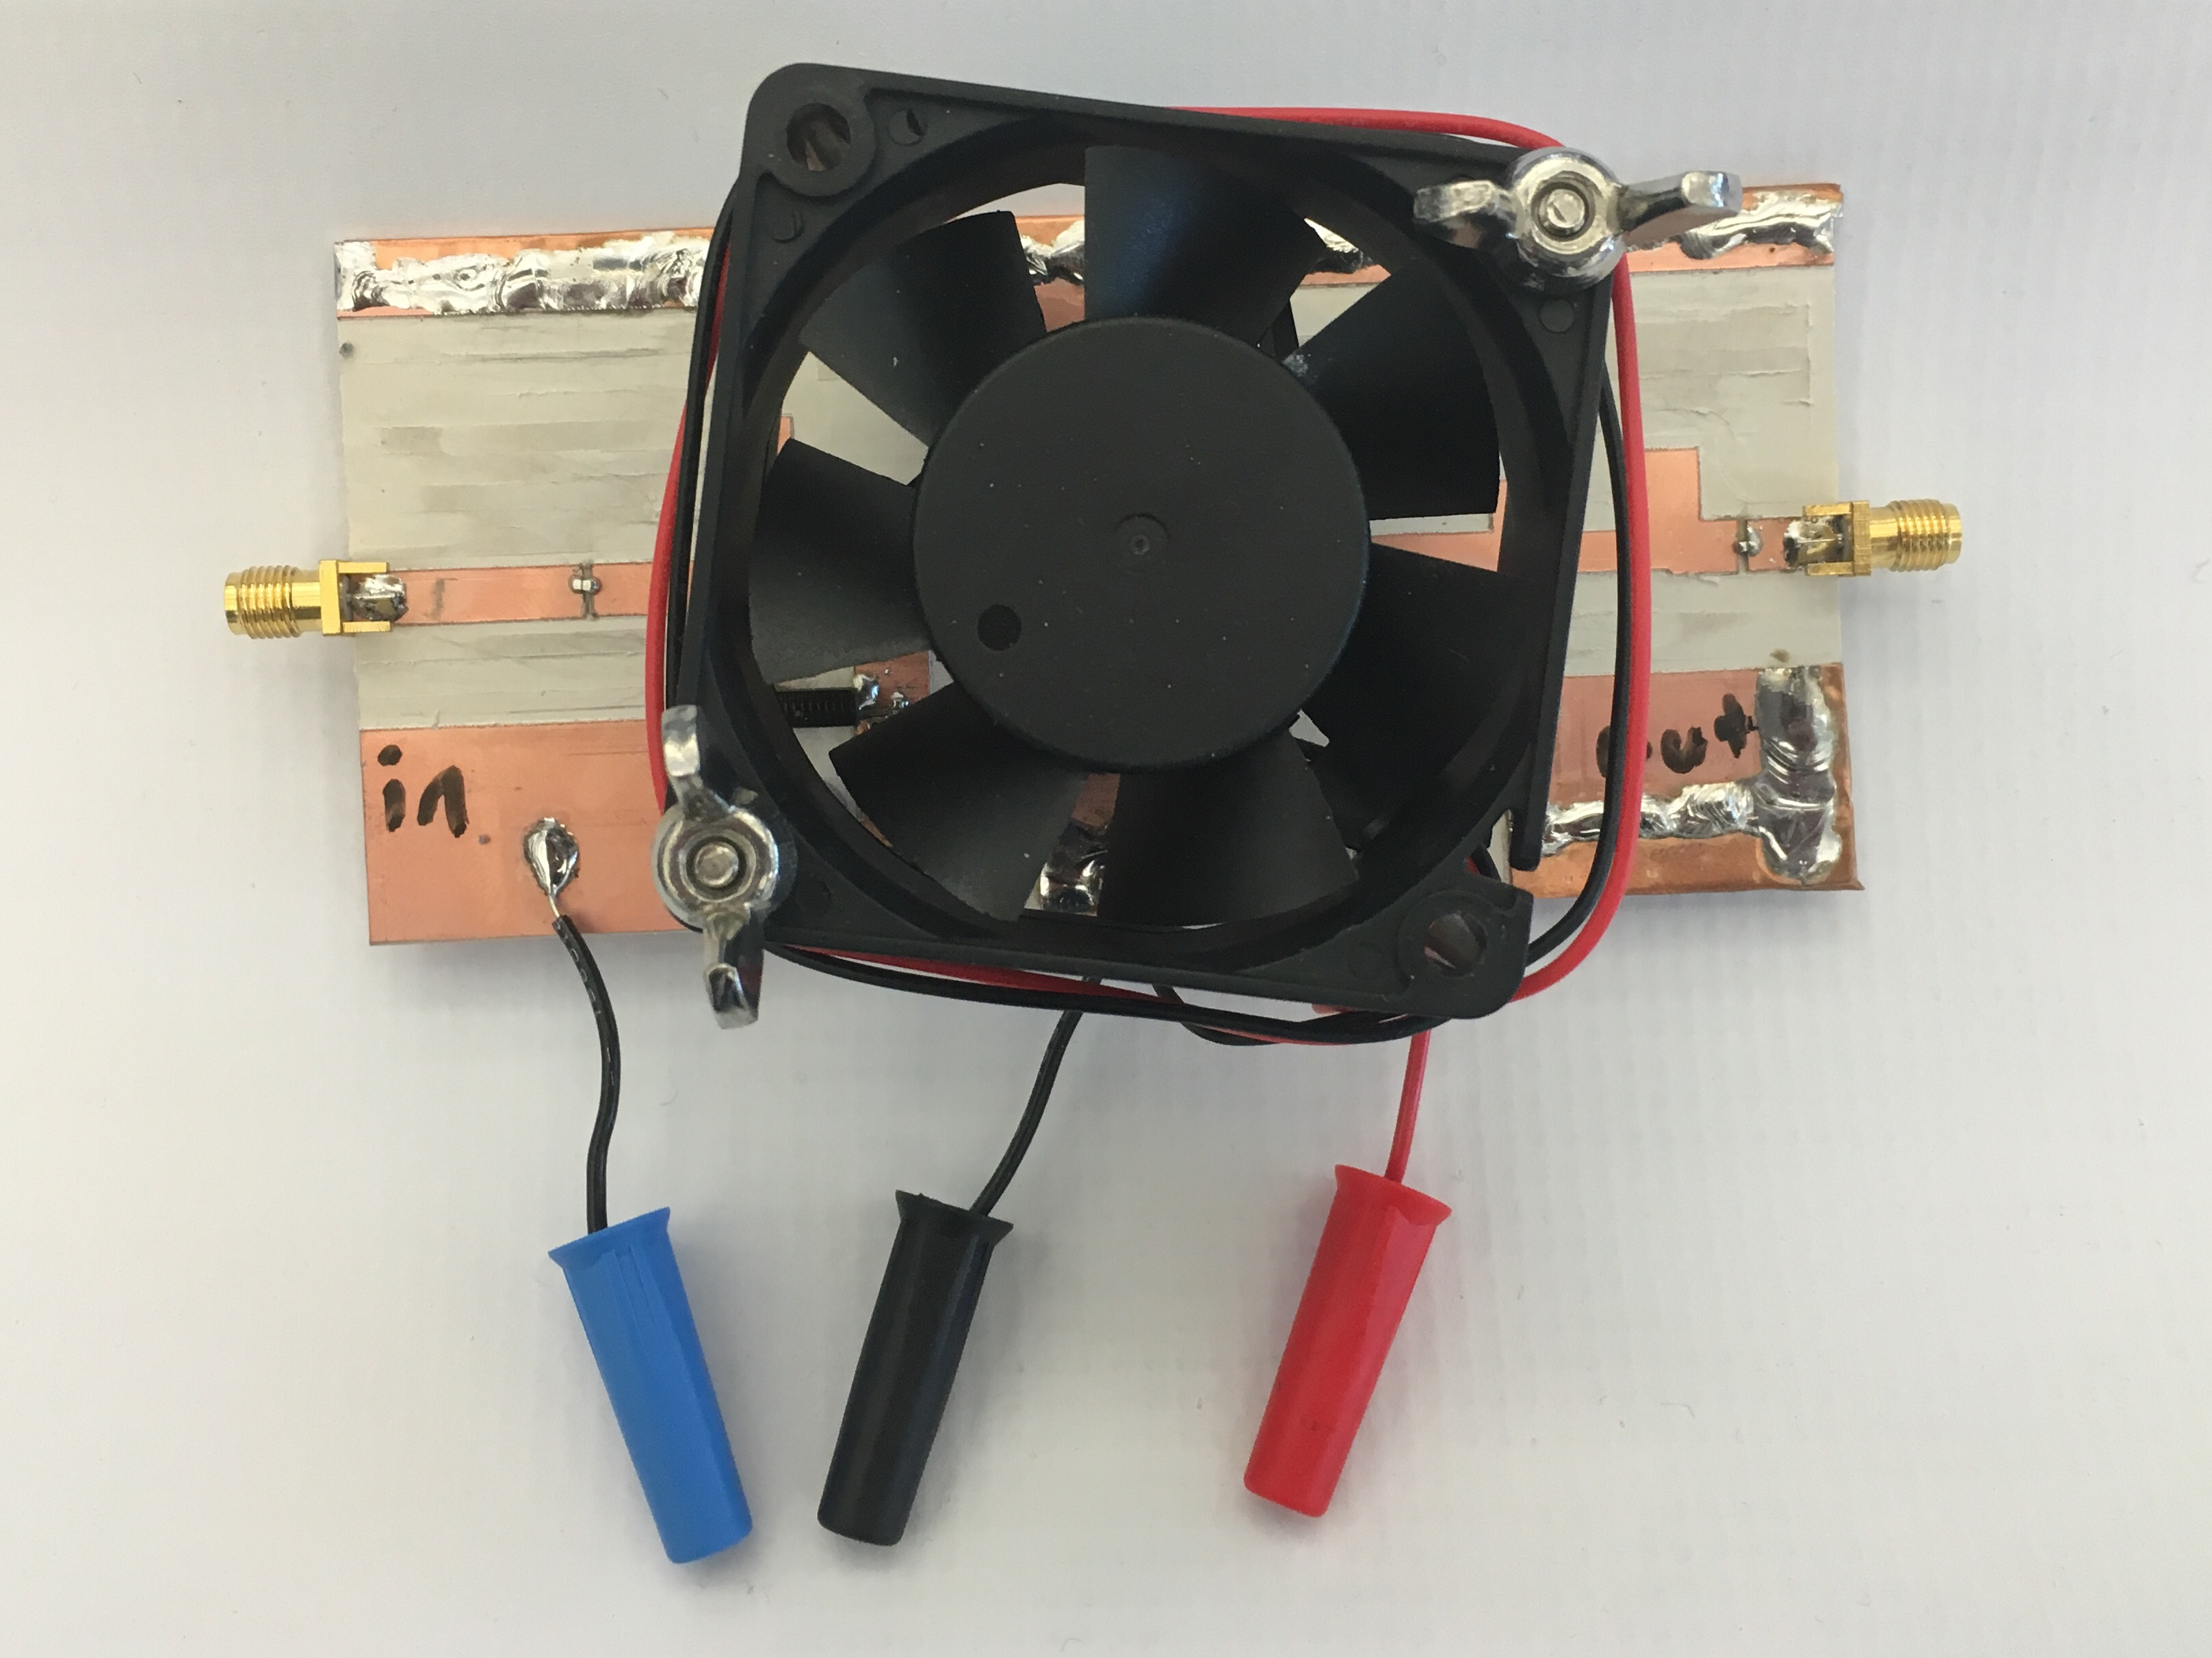
\includegraphics[width=5in,height=5in,keepaspectratio]{figures/test/final_fan}\\
  \caption{Photo of Final Amplifier With the Fan}
  \label{fig:final_fan}
\end{figure}

The bias network for the final amplifier used grounded shunt caps on the quarter wavelength stubs to create RF shorts. The DC bias was then fed through the quarter wavelength stubs through a series wideband spiral inductor. Two previous versions of the amplifier were built but due to the challenge of soldering the leadless package of the transistor they were damaged most likely due to shorts and insufficient cooling. The bias inductors, coupling capacitors, and transistor was mounted on the board using solder paste and a heatgun. SMA connectors were soldered on the input and output traces and banana plugs were soldered to the DC bias pads to comply with the competition rules. The final build of the amplifier without the fan can be seen in Figure \ref{fig:final_amp} and with the fan in Figure \ref{fig:final_fan}. The amplifier was measured with an Anritsu MS4622B and the drain powered with an Agilent Power Supply E3640A with the drain current being measured by an Agilent Multimeter Agilent U3606A. The gate voltage was powered by an Agilent Power Supply E3630A. After tuning the gate bias and measuring the amplifier performance, a final gate voltage of -2.66 V for the amplifier. A photo of the test setup can be seen in Figure \ref{fig:test_setup}.

%A bill of materials and the board layout can be found in the Appendix.

%Fix VNA part number

%A drain current versus drain-source voltage measurement at a gate voltage of -2.6 V can be seen in Figure X.

For the RF measurements the VNA was calibrated from 2 GHz to 4 GHz and set to average ten samples. A 20 dB attenuator was put at the output of the amplifier so the VNA would not be damaged by the high RF output power. The 20 dB attenuator was measured so the attenuation could be removed and the amplifier gain could be properly measured. The measured center frequency of the final amplifier was 2.91 GHz and the various measured parameters of the amplifier can be seen in Figure \ref{fig:meas_singlesweep}. The VNA used to measure the amplifier was only able output a maximum of 20 dBm of power compared to the competition maximum of 24 dBm input power which limits the maximum PAE the amplifier can achieve.

\begin{figure}
  \centering

  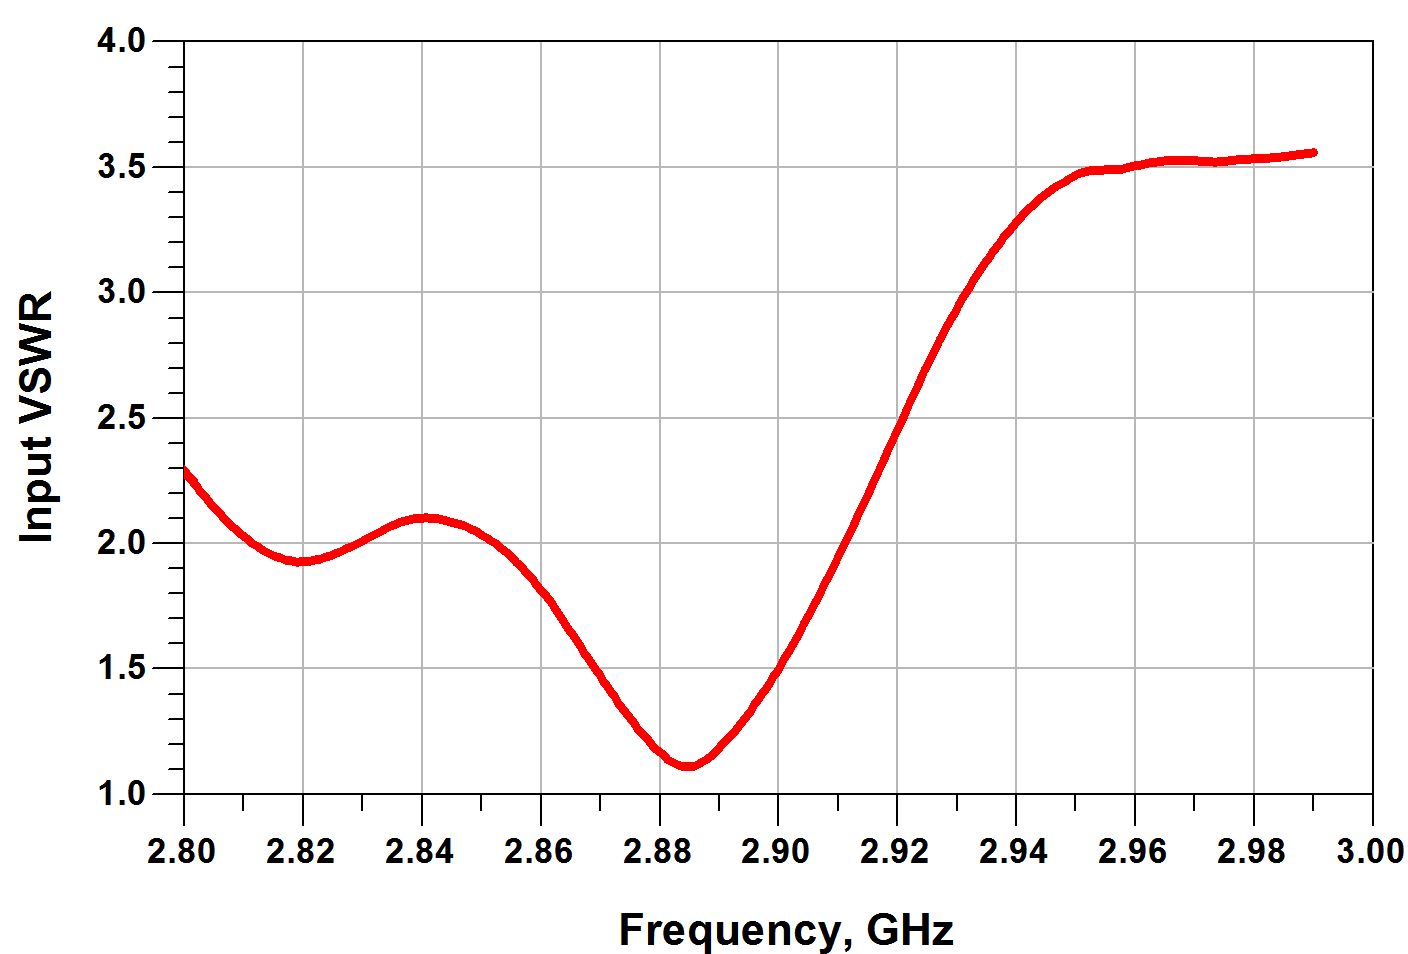
\includegraphics[width=5in,height=5in,keepaspectratio]{figures/test/input_vswr}\\
  \caption{Measured Input VSWR of Final Amplifier}
  \label{fig:input_vswr}
\end{figure}

 The amplifier s-parameters and drain current was measured over a wide range of input powers from -30 dBm to 20 dBm. Only the input VSWR seen in Figure \ref{fig:input_vswr} could be measured properly. The 20 dB attenuator at the output resulted in erroneous output VSWR when de-embedded which is most likely due to the reflection from the attenuator being larger than the reflection from the output of the amplifier. The amplifier had the best input match at slightly below the center frequency at 2.89 GHz with a VWSR of 1.11 and at the center frequency of 2.91 GHz the VSWR was measured to be 1.9.

 \begin{figure}
  \centering
  % Requires \usepackage{graphicx}
  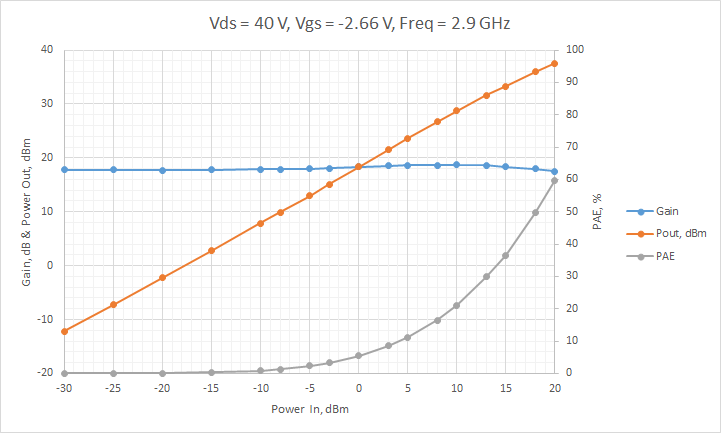
\includegraphics[width=5in,height=5in,keepaspectratio]{figures/test/meas_singletone}\\
  \caption{Measured Parameters of Final Amplifier}
  \label{fig:meas_singlesweep}

\end{figure}

 The final amplifier was able to output a maximum of 37 dBm at an input power of 20 dBm and a PAE of 59.8\% resulting in a figure of merit of 78. The amplifier is able to output 36 dBm at input powers 18 dBm or greater which is 3 dB more than the design goal. The amplifier most likely has a maximum PAE in the 70\% range at the maximum allowed input power of 24 dBm from looking at the increase in input power from 15 dBm to 20 dBM, the PAE increases from 36\% to 60\%. The amplifier has 19 dB of gain from -30 dBm to 15 dBm of input power and shows gain compression beyond 15 dBm seen in Figure \ref{fig:meas_singlesweep}.

 To qualify for the IMS competition the amplifier carrier-to-interference (C/I) ratio must be greater than 30 dB using two 5 MHz spaced tones at an input power of 0 dBm. The C/I was measured by taking an intermodulation distortion measurement of the amplifier from 2.8 GHz to 3 GHz seen in Figure \ref{fig:meas_imd}. The IMD was well below the required 30 dB and was around -80 dB across the entire frequency band. The output third order intercept (OIP3) was calculated using the IMD measurement, and can be shown in Figure \ref{fig:output_ip3}. At the center frequency of 2.9 GHz the OIP3 is around 55 dBm.

 A comparison of the amplifier measurements and the design specifications can be seen in Table \ref{table:meas_spec_compare}. It should be reiterated that it was expected the fabricated amplifier would require a higher input power than the design specification to take in account non-idealities that could not be taken into account in the simulation. The amplifier has a lower center frequency than expected but at a fixed PAE it amounts to less than a one point difference in the figure of merit. Overall while the amplifier may not have met all of the design specifications, it is still a functional class F amplifier that can compete in the design competition.

 %Table comparing the final design specs to the measurements
\begin{table}
    \centering
    \caption{Comparison of the Specification and Measured Performance of Amplifier}
    \label{table:meas_spec_compare}
    \begin{tabular}{|l|l|l|}
      \hline
      % after \\: \hline or \cline{col1-col2} \cline{col3-col4} ...
      {Parameter}                      & {Specification }   & {Measured} \\ \hline
      {Center Frequency, GHz}          & 3                  & 2.9 \\ \hline
      {Input Power for Max PAE, dBm}    & 15                 & 20 \\ \hline
      {Output Power for Max PAE, dBm}  & {\textgreater 36}  & {37} \\ \hline
      {Maximum PAE, \%}                & 70                 & {59.8} \\ \hline
      {Input and Output VSWR}          & {\textless 2}      & {\textless 2} \\ \hline
    \end{tabular}
\end{table}

 \begin{figure}
  \centering
  % Requires \usepackage{graphicx}
  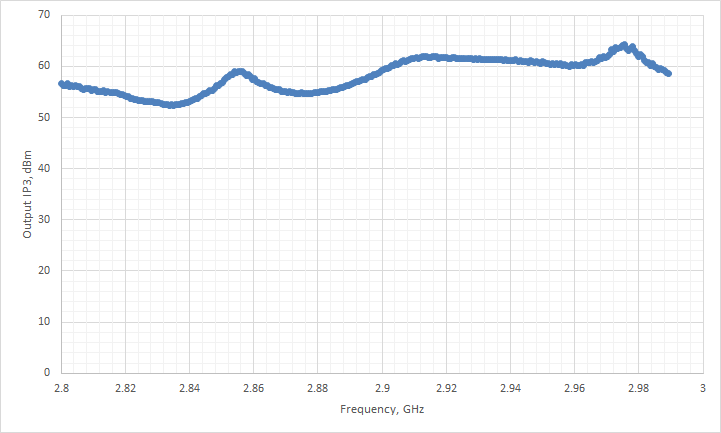
\includegraphics[width=5in,height=5in,keepaspectratio]{figures/test/output_ip3}\\
  \caption{Measured Output Third Order Intercept of Final Amplifier}
  \label{fig:output_ip3}
\end{figure}

\begin{figure}

  \centering
  % Requires \usepackage{graphicx}
  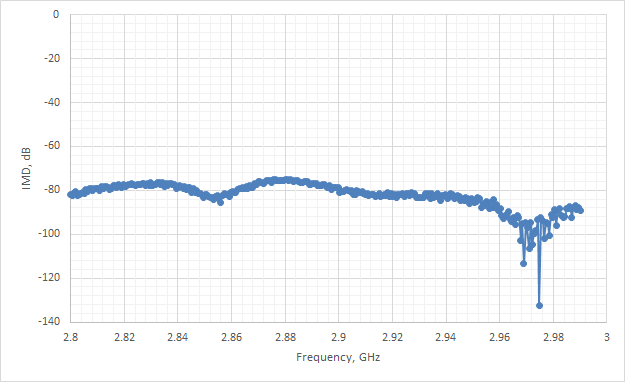
\includegraphics[width=5in,height=5in,keepaspectratio]{figures/test/meas_imd}\\
  \caption{Measured Intermodulation Distortion of Amplifier Using 2 Tones 5 MHz Apart}
  \label{fig:meas_imd}
\end{figure}

A major challenge of the thesis was finding equipment to measure the amplifier. Only one of the signal generators in the microwave laboratory was able to output 24 dBm at 3 GHz. Some of the equipment that was rated to output the RF power needed to measure the amplifier was measured on signal analyzers to be much less. No equipment was able to do the two tone test at a high power and will have to be done at the conference. The two-tone intermodulation distortion measurement had to be done on the Antritsu MS4622B VNAs which had a maximum output power of 7 dBm. Fortunately to qualify for the competition, the carrier-to-interference (C/I) specification of greater than 30 dB at 0 dBm input power was able to be measured.

\begin{figure}
  \centering
  % Requires \usepackage{graphicx}
  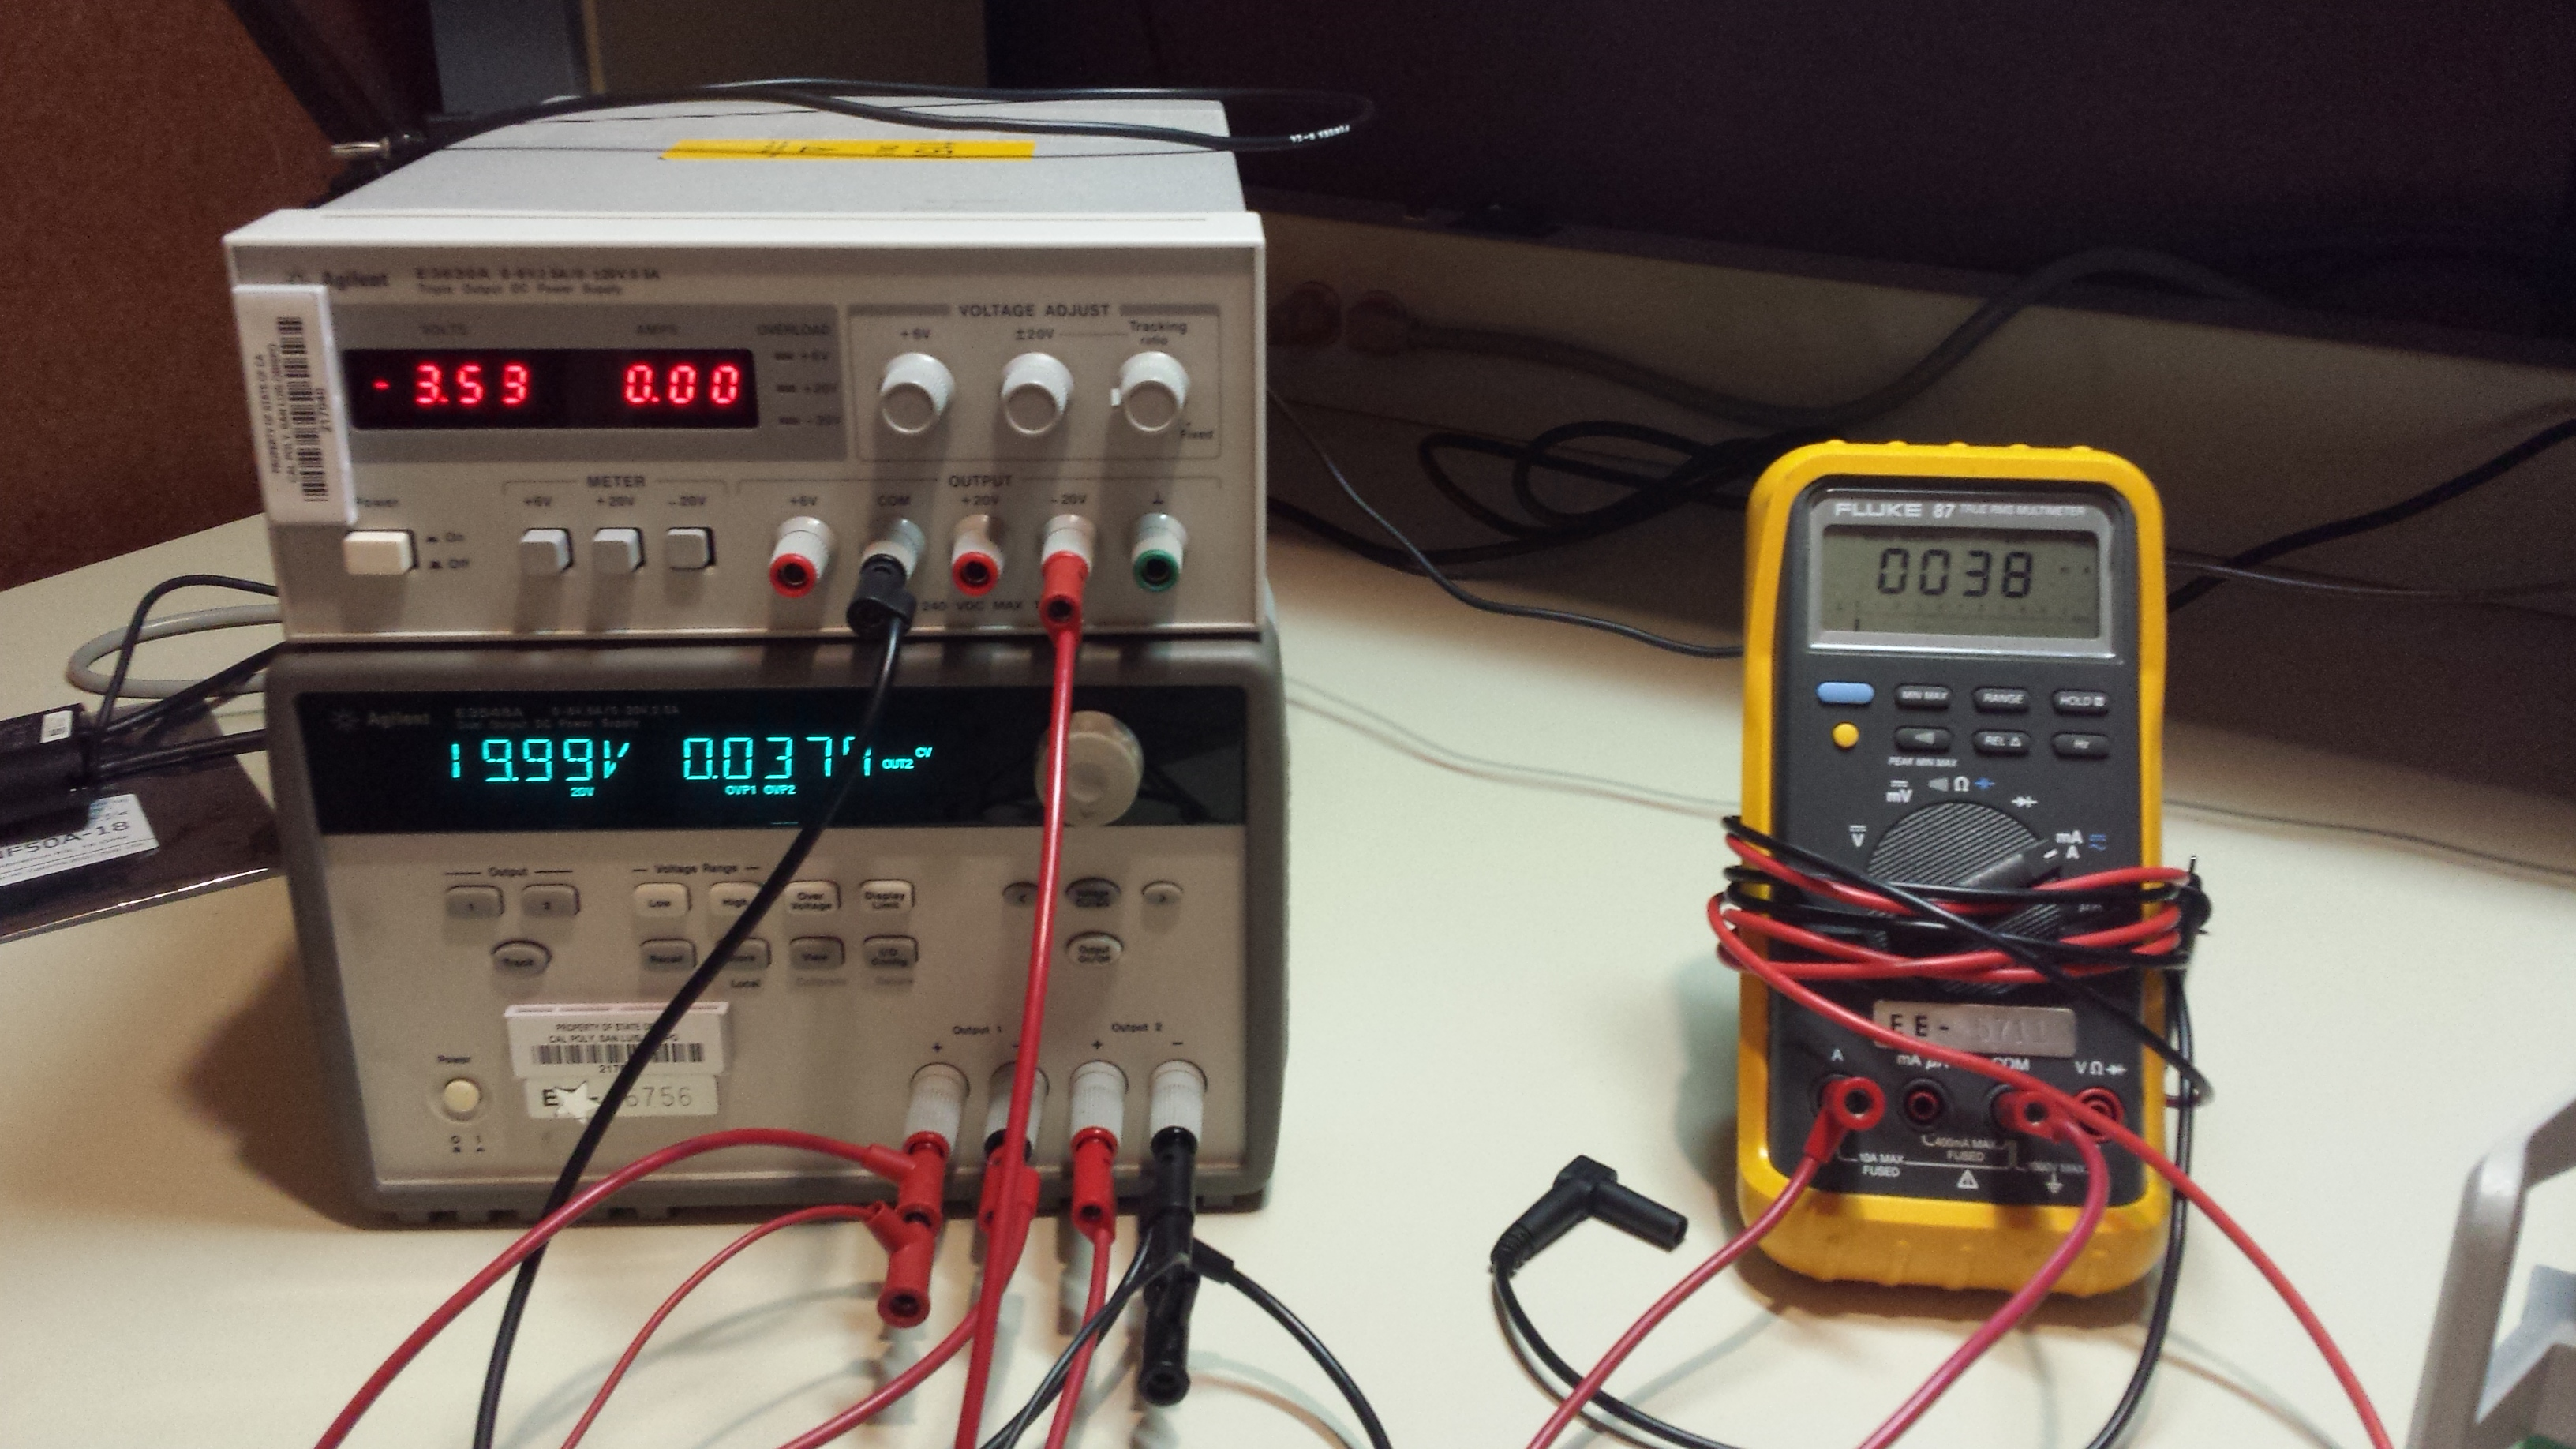
\includegraphics[width=5in,height=5in,keepaspectratio]{figures/test/test_setup}\\
  \caption{Photo of Test Setup}
  \label{fig:test_setup}
\end{figure}

  %\vspace*{\floatsep}
\begin{figure}
  \centering
  % Requires \usepackage{graphicx}
  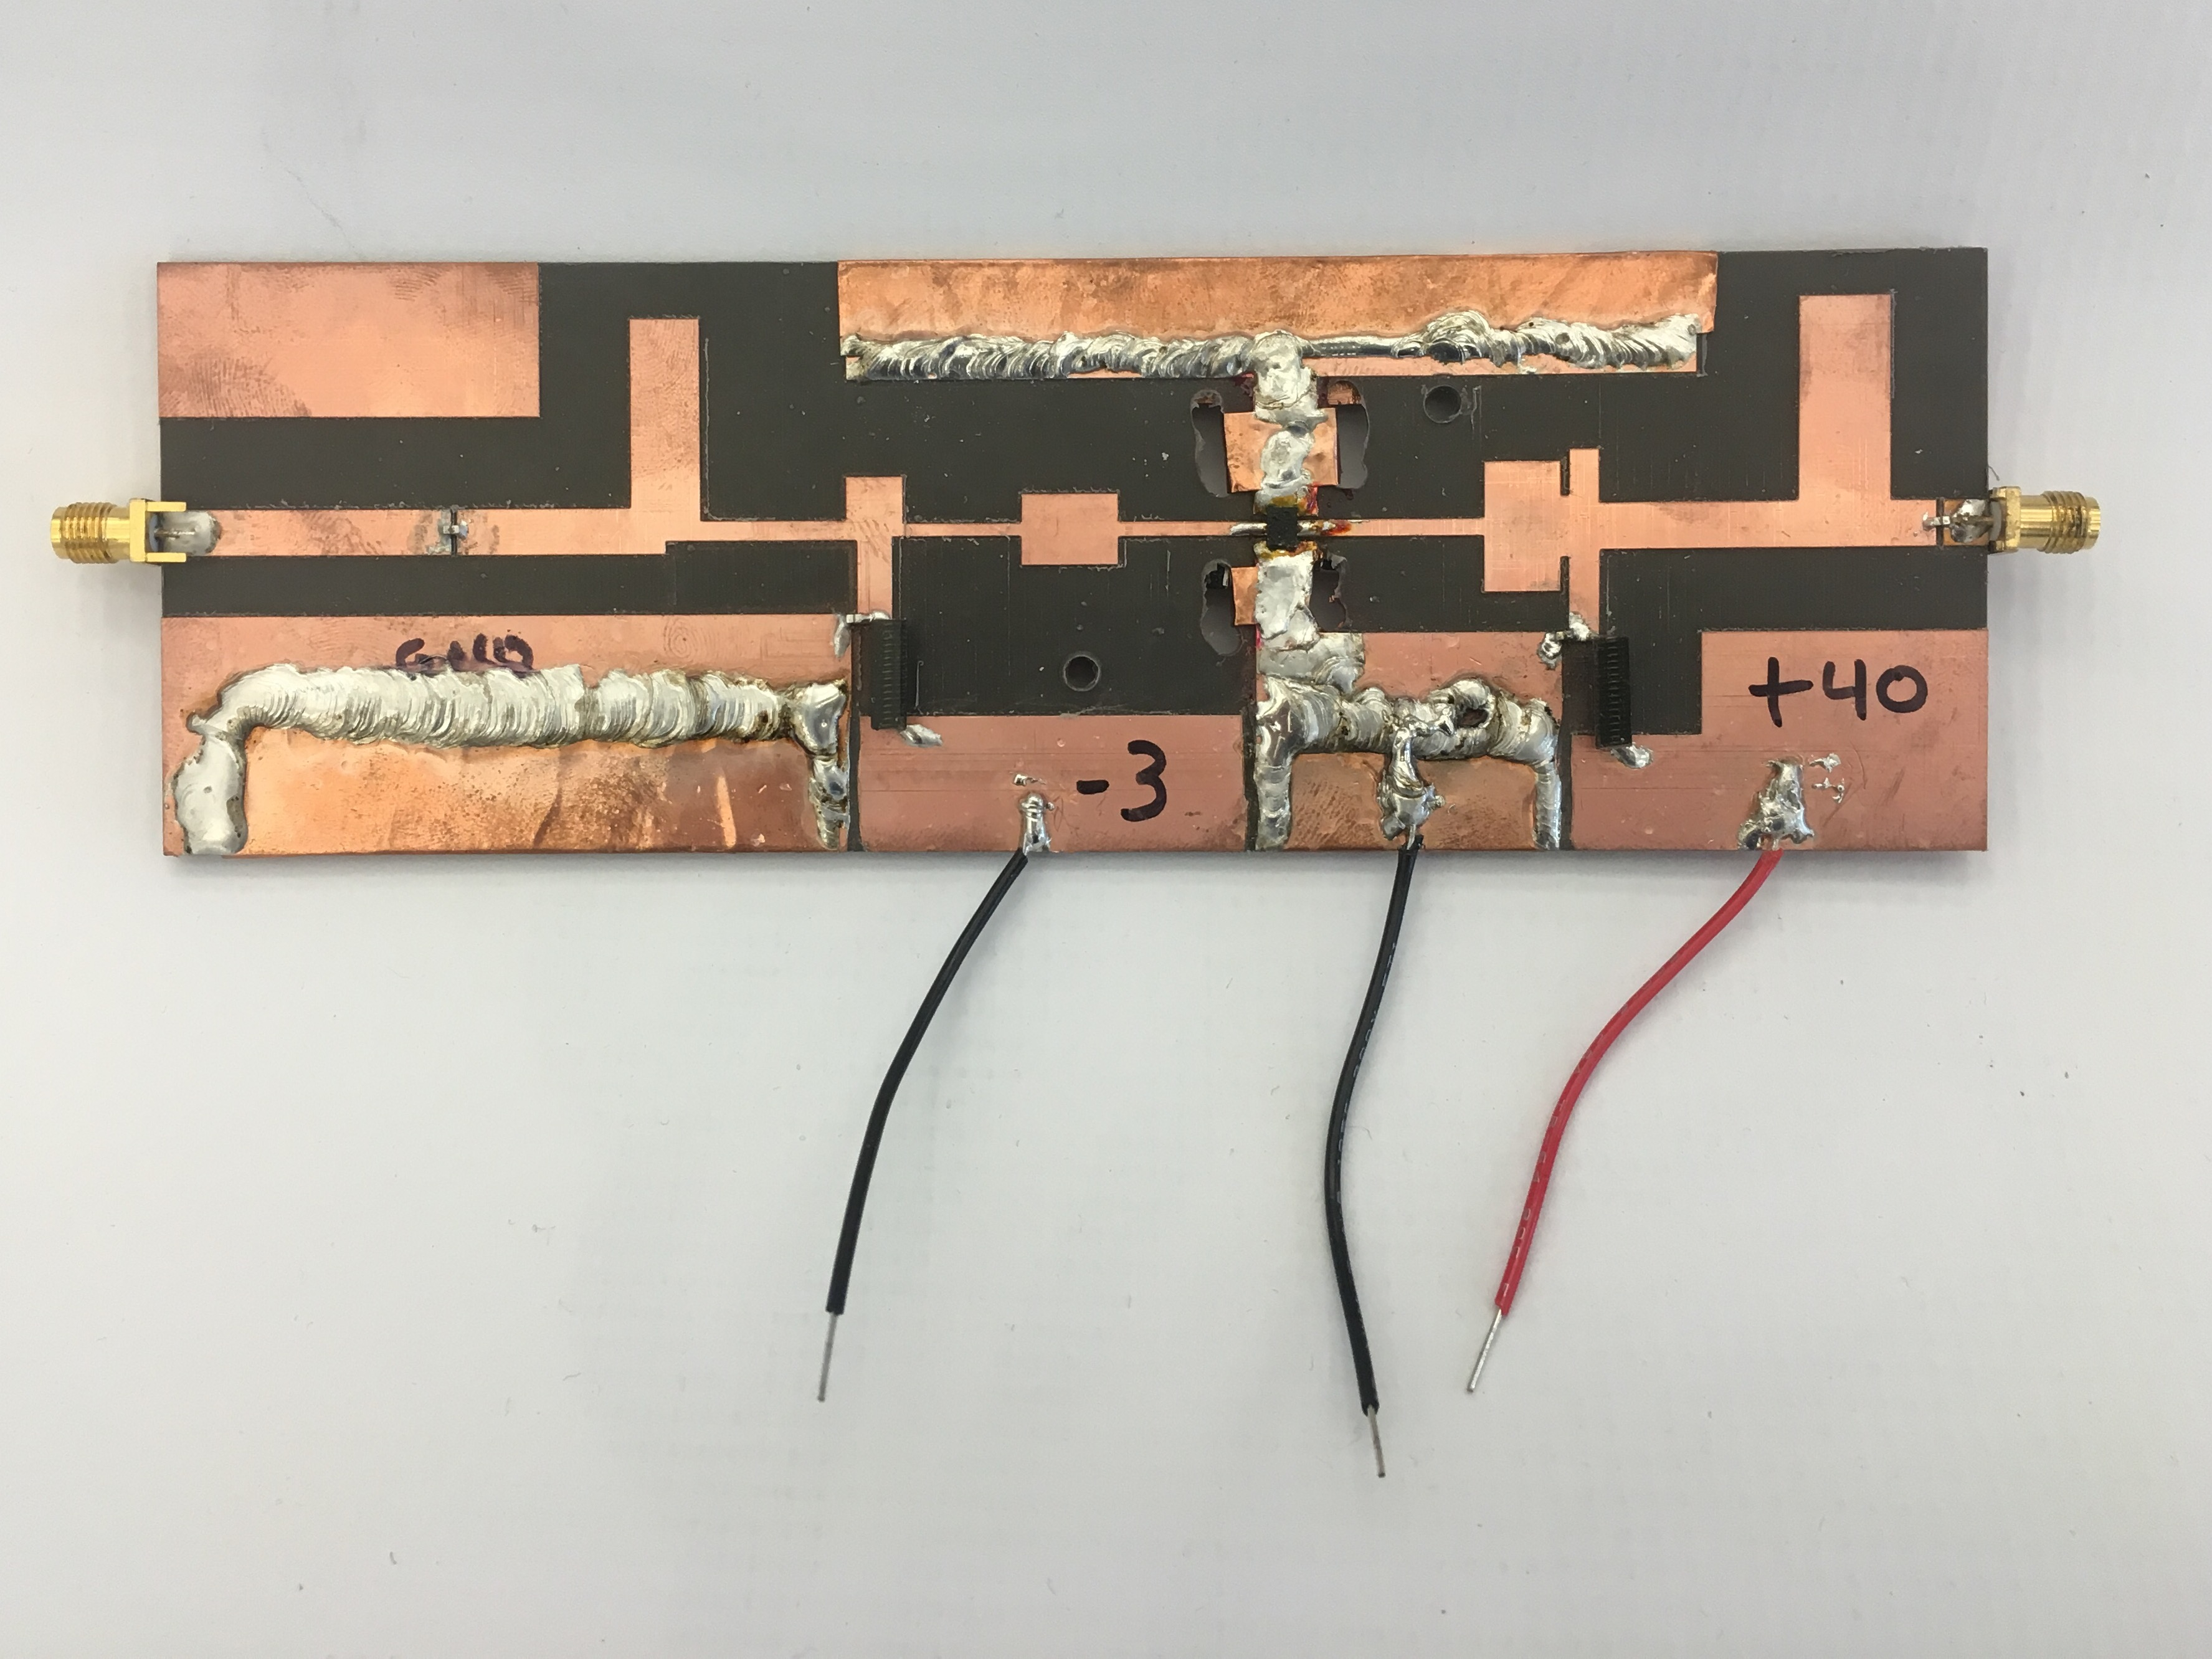
\includegraphics[width=5in,height=5in,keepaspectratio]{figures/test/old_amp}\\
  \caption{Photo of Previous Version of Amplifier}
  \label{fig:old_amp}
\end{figure}

%
%\chapter{Conclusion, Future Projects} 




\clearpage
\begin{flushleft}
\nocite{*}
\bibliography{library}
\bibliographystyle{plain}
\end{flushleft}

\begin{appendices}


\end{appendices}

\end{document}
